\subsection{Fenêtres homologues du chromosome humain}
Les fenêtres homologues proviennent du chromosome~21 de GRCh38.p14 (\texttt{NC\_000021.9}) et de T2T-CHM13v2.0 (\texttt{NC\_060945.1})~\cite{grch38,t2t,chmreleases}. Sur le chromosome 21, les intervalles commencent en 34\,000\,000 et 32\,381\,795, en coordonnées de base zéro. Les ancres de 41 bases qui encadrent chaque intervalle sont uniques sur leur chromosome. La chaîne de correspondance UCSC de \texttt{hg38} vers \texttt{hs1}~\cite{ucscchain} place leurs extrémités dans le même ordre sur le brin positif. Les insertions et les délétions internes restent dans les fenêtres.
\chart{biology/chromosome21.png}{Chaque ligne associe le temps et la mémoire d’un alignement. Les hachures indiquent le maximum résident échantillonné et les barres pleines, le pic système.}{fig:humain}{bench/human/human.sbatch}
Dans la figure~\ref{fig:humain}, cinq processus par méthode alignent les mêmes fenêtres après un premier appel complet. Pour deux puis quatre millions de bases de référence, les distances valent \(5\,599\) et \(12\,482\). La portée \(R\) de l'index atteint 290 puis 622 colonnes, ce qui impose un lancement CUDA par ligne. NvPD prend \(17{,}558\pm0{,}115\) puis \(90{,}420\pm0{,}276\)\,s, allocations, transferts et synchronisation compris. L'initialisation du contexte a lieu pendant l'échauffement. Pour les mêmes fenêtres, WFA2 sur un cœur Grace prend \(0{,}0539\pm0{,}0006\) puis \(0{,}3455\pm0{,}0019\)\,s, et edlib \(0{,}7864\pm0{,}0079\) puis \(2{,}9980\pm0{,}0013\)\,s.

La mémoire hôte est mesurée dans cinq processus par méthode. À quatre millions de bases, le pic RSS du processus CUDA vaut 252\,Mio. Les compteurs de pic des bibliothèques Grace restent à zéro dans le premier relevé. Un second passage échantillonne leur RSS environ chaque milliseconde. Les maxima observés, bornes inférieures du pic réel, valent \(24{,}125\pm0{,}000\)\,Mio pour edlib et \(20{,}988\pm0{,}028\)\,Mio pour WFA2. Les tampons explicitement réservés sur le GPU sont comptés à part.

Le contrôle entier ajoute 64 bases à une copie des 45\,090\,682 bases de CHM13. Le chemin construit coûte 64 et la différence de longueur impose \(d\ge64\). WFA2 obtient ce score en \(10{,}74\pm0{,}09\)\,ms à chaud sur Grace en cinq blocs.

\synthese{Sur les fenêtres de deux et quatre millions de bases, les portées maximales des prédécesseurs valent 290 et 622 colonnes. Elles dépassent la limite du halo, ce qui impose le noyau par ligne sur ces deux entrées.}

\subsection{Comparaison des assemblages chromosomiques entiers}
Les versions v1.0 et v2.0 de CHM13 permettent de mesurer le coût d'une révision d'assemblage sur le chromosome 20. Les entrées \texttt{CP068258.1} et \texttt{CP068258.2} comptent 66\,210\,247 et 66\,210\,255 bases~\cite{chmreleases}. Le chromosome 20 porte déjà l'accession \texttt{CP068258.2} dans la version intermédiaire 1.1. Sur le chromosome 21, GRCh38 et CHM13 représentent deux références distinctes et comportent des bases ambiguës traitées comme des caractères ordinaires.

Une borne exploite l'histogramme des lettres, où \(f_A(c)\) désigne l'effectif de la lettre \(c\) dans \(A\). Pour \(u_c=f_A(c)-f_B(c)\) et \(x_+=\max(0,x)\), chaque édition efface au plus une unité d'excédent et une de déficit. Ainsi,
\[
 d(A,B)\ge\max\!\left(\sum_c(u_c)_+,\ \sum_c(-u_c)_+\right).
\]
Une borne supérieure suit un alignement global réalisable. Sur chaque bloc de la chaîne UCSC 23, il paie les désaccords. Dans chaque intervalle entre blocs, il choisit le moins coûteux des deux alignements ancrés à gauche ou à droite, puis paie l'écart de longueur. Les extrémités suivent la même règle. La somme des coûts des blocs et des intervalles donne le coût du chemin entier.
\chart{biology/chromosomes_entiers.png}{Les durées sur le chromosome 20 et les bornes de distance sur le chromosome 21 comparent deux niveaux de divergence entre assemblages.}{fig:chrentiers}{bench/human/whole_chromosomes.py}
Le panneau des temps de la figure~\ref{fig:chrentiers} porte sur cinq blocs à chaud sur un cœur Grace. Les deux bibliothèques donnent \(d=30\) sur le chromosome 20. Edlib prend \(0{,}9767\pm0{,}0026\)\,s et WFA2 \(0{,}01644\pm0{,}00012\)\,s. Pour le chromosome 21, les appels de la campagne EPYC ont tous atteint la limite murale de 120\,s. L'écart de longueur seul vaut 1\,619\,301 bases.

Sur le chromosome 20, un chemin optimal donne \(N_{\mathrm{sub}}=18\), \(N_{\mathrm{ins}}=10\) et \(N_{\mathrm{del}}=2\). Leur somme vaut 30, tandis que les huit bases de différence de longueur correspondent à \(10-2\). Sur ce chemin, 19 éditions précèdent un bloc identique de 66\,209\,720 bases et 11 le suivent. Les intervalles de base zéro, fin exclue, sont \(A[270,66\,209\,990)\) et \(B[277,66\,209\,997)\). Le bloc couvre 99,999204\,\% de la première version. Cette localisation décrit une révision d'assemblage et l'un des chemins optimaux possibles. Le consortium T2T signale une amélioration du polissage des régions télomériques entre les versions 1.0 et 1.1~\cite{chmreleases,mccartney}. Les coordonnées du chemin ne suffisent pas pour attribuer chaque édition à une correction particulière. La figure~\ref{fig:chrentiers} situe les opérations par rapport au bloc commun.

\synthese{Pour le chromosome 21 entier, la composition et un chemin réalisable encadrent la distance entre 6\,621\,364 et 16\,015\,052 éditions. Le score exact reste inconnu après les arrêts à l'échéance.}

\subsubsection{Éditions entre deux versions du génome humain}\label{sec:panelhumain}
Les versions v1.0 et v1.1 de T2T-CHM13 décrivent le même échantillon humain. La v1.1 améliore le polissage des extrémités et comble cinq lacunes dans les répétitions de l'ADN ribosomique~\cite{chmreleases,mccartney}. L'expérience porte sur les 17 autosomes qui ne portent pas ces lacunes et sur le chromosome X. Elle compare chaque chromosome entier à son homologue, dans le sens déposé.

Pour une paire de longueurs \(m,n\), un chemin optimal vérifie
\[
 n-m=N_{\mathrm{ins}}-N_{\mathrm{del}},\qquad
 d-|n-m|=N_{\mathrm{sub}}+2\min(N_{\mathrm{ins}},N_{\mathrm{del}}).
\]
La différence de longueur donne ainsi un nombre minimal d'insertions ou de délétions, même lorsque plusieurs chemins ont le même score. La figure~\ref{fig:panelhumain} rapporte les scores par chromosome et les temps sur un cœur EPYC. Chaque processus effectue un échauffement sur la paire complète avant la mesure. La lecture FASTA précède le chronométrage.

\chart{biology/cohorte_chromosomes.png}{Les distances et les temps d'alignement portent sur les mêmes dix-huit chromosomes entre les versions v1.0 et v1.1 de CHM13.}{fig:panelhumain}{bench/human/chromosome-panel/measure.py}
Sur le chromosome~1, la première version mesure 248\,387\,497 bases. Pour ses 176 éditions, WFA2 prend \(0{,}119\pm0{,}049\)\,s contre \(5{,}418\pm0{,}028\)\,s pour Edlib. Sur le chromosome~3, plus court, la distance atteint 659 et Edlib prend \(9{,}129\pm0{,}082\)\,s. Les durées de WFA2 varient davantage entre processus. Sur quinze chromosomes, la demi-largeur de l'intervalle à 95\,\% dépasse 5\,\% de la moyenne.

Le consortium recense 310 changements sur ces chromosomes dans un fichier VCF.\footnote{Chaque entrée VCF indique une position sur la séquence de référence et les allèles à cet endroit.} Parmi eux, 292 tiennent dans les mille premières ou dernières bases du chromosome. Le remplacement littéral des allèles reproduit la v1.1 sur quatorze chromosomes. La commande \texttt{consensus} de BCFtools~1.21~\cite{bcftools} rend les mêmes séquences que le rejeu. Sur les quatre autres, seule la première base diffère encore. En incluant ces quatre substitutions, le chemin décrit par le fichier coûte 2\,667 éditions, soit 80 de plus que le minimum global. Plusieurs changements voisins peuvent admettre un alignement commun moins coûteux.

\synthese{Les deux bibliothèques trouvent au total 2\,587 éditions sur 2\,643\,920\,725 bases de la version v1.0. Les écarts de longueur imposent au moins 2\,330 insertions ou délétions, soit 90,1\,\% du coût cumulé.}

\subsection{Localisation des révisions de l’assemblage humain}\label{sec:paysage-chromosomique}
Pour situer les révisions entre les versions v1.0 et v1.1 de CHM13, on relève l’intervalle de référence \([a_i,b_i)\) de chaque entrée du VCF du consortium~\cite{chmreleases,mccartney}. Sur un chromosome de longueur \(L_i\), la plus petite marge terminale qui contient l’intervalle entier a pour largeur \(r_i=\min(b_i,L_i-a_i)\). La figure~\ref{fig:paysage-chromosomique} cumule les entrées en fonction de cette largeur,
\[
 F_w(h)=\frac{\sum_i w_i\,\mathbf{1}_{r_i\le h}}{\sum_i w_i}.
\]
Le poids \(w_i=1\) compte chaque entrée une fois. Le poids \(w_i=d(\mathrm{REF}_i,\mathrm{ALT}_i)\) mesure le coût du remplacement de son allèle. Le total de 2\,663 éditions couvre les allèles consignés dans le VCF. Les quatre substitutions résiduelles du rejeu interviennent séparément dans la borne de la section~\ref{sec:panelhumain}.

\chart{biology/paysage_chromosomique.pdf}{Le panneau a) donne la part des 310 entrées et de leur coût couverte par des marges de 0 à 1\,000~nt. Le panneau b) répartit ce coût entre les deux marges de 500~nt et les autres entrées de chaque chromosome. Les cases blanches ont un coût nul.}{fig:paysage-chromosomique}{python/studies/chromosome_landscape.py}
\FloatBarrier
\Needspace{4\baselineskip}
La marche à 492~nt correspond à une délétion de 491 bases au début du chromosome~3. Cet allèle représente à lui seul 18,4\,\% du coût du VCF sur le panel. À l’autre bout de la distribution, une substitution sur le chromosome~9 exige une marge de plus de 16~Mnt. Le découpage des chromosomes doit donc aussi tenir compte de révisions intérieures.

\synthese{Sur les 18 chromosomes, les 500 bases de chaque extrémité couvrent 18\,000 des 2\,643\,920\,725 bases de référence. Elles contiennent 263 des 310 entrées, soit 84,8\,\% des entrées et 98,2\,\% de leur coût.}

\subsubsection{Calcul par fronts sur les révisions d’un haplotype}
Les révisions v1.1 et v1.2 de HG002 permettent de mesurer l’effet de quelques éditions dispersées sur un chromosome entier~\cite{hg002,hg002data}. Chaque comparaison porte sur deux versions du même haplotype. Les séquences du chromosome 1 comptent de 244 à 252 millions de bases. Sur le chromosome 21, l'assemblage maternel conserve 3\,671\,963 symboles N et le paternel 2\,300\,690. Ces lacunes d’assemblage restent dans le calcul, avec un coût nul pour N face à N. L’application des 67 entrées du VCF aux quatre séquences v1.1 restitue les quatre séquences v1.2.

Dans les fragments de la figure~\ref{fig:split}, les longues plages identiques peuvent se parcourir directement. Pour un budget d’éditions \(s\) et une diagonale \(k=i-j\), le front \(F_s(k)\) mémorise le plus grand indice \(i\) atteint. La délétion, la substitution et l’insertion donnent les trois candidats~\cite{ukkonen,wfa},
\[
 x=\max\{F_{s-1}(k-1)+1,\;F_{s-1}(k)+1,\;F_{s-1}(k+1)\},
 \qquad F_s(k)=x+\operatorname{LCP}(A_{x:},B_{x-k:}).
\]
Les transitions sortant du rectangle sont écartées. Le préfixe commun initialise \(F_0(0)\). Le premier front qui atteint \((m,n)\) donne la distance minimale. Pour le score seul, la commande \texttt{nvpd-sparse} conserve les coupes vérifiées et NvPD pour les petits rectangles. Dans les grands, elle explore jusqu’à 128 éditions par fragment avant de passer à BiWFA. Deux tableaux de 259 entiers occupent 2\,072 octets par travailleur. L’extension lit les deux séquences par blocs de 4\,096 puis de 64 octets.

Le panneau a) de la figure~\ref{fig:hg002-dispatch} compare les solveurs sur un cœur EPYC. Dans chacun des cinq blocs, un processus par méthode effectue un appel de chauffe puis un appel chronométré, après lecture des séquences.

Lorsqu’une coupe est rejetée, les fragments adjacents doivent être réunis. Les bases déjà reconnues comme identiques aux deux extrémités du groupe restent appariables. Pour des chaînes \(P,X,Y,S\), la distance unitaire vérifie
\[
 d(PXS,PYS)=d(X,Y).
\]
Le programme conserve la longueur des extrémités communes de chaque fragment. Il enlève les fragments terminaux de score nul, puis les extrémités communes des fragments restants. S’il ne reste qu’un fragment, son score est déjà connu. Le panneau b) isole l’effet de cette réutilisation à nombre de cœurs fixé. Pour chaque chromosome, un même processus exécute un bloc de chauffe puis sept blocs en ordre aléatoire.
\chart{comparison/chromosome_dispatch.pdf}{Le panneau a) rapporte le temps de WFA2 à celui des solveurs sur un cœur, avec l’écart-type et l’IC à 95\,\% de cinq rapports appariés. Le panneau b) rapporte le temps avec relecture à celui avec réutilisation, pour un et huit cœurs. Le symbole indique la moyenne, le trait épais un écart-type et le trait fin les extrêmes des sept blocs.}{fig:hg002-dispatch}{python/studies/chromosome_dispatch.py}
Sur le chromosome 1 maternel, le score vaut 54. À un cœur, le temps passe de \(157{,}05\pm0{,}47\) à \(28{,}19\pm0{,}06\)\,ms lorsque le découpage utilise le front borné. WFA2 prend \(87{,}18\pm0{,}80\)\,ms et Edlib \(4{,}393\pm0{,}031\)\,s. Le pic résident moyen du processus descend de 834 à 477\,Mio entre les deux variantes du découpage, FASTA compris. Les compteurs en mode utilisateur relèvent 59,6 millions d’instructions contre 334,3 millions. Le nombre de défauts de lecture L1 passe de 38,89 à 11,03 millions, alors que leur part dans les lectures monte de 23,3 à 35,6\,\%.

Sur le chromosome~1 paternel, une des sept coupes proposées entraîne une fusion. À huit cœurs, la réutilisation ramène le temps de \(21{,}07\) à \(10{,}76\)\,ms. Sur le chromosome~1 maternel, une coupe est également rejetée et le gain moyen vaut 1,054. Sur le chromosome~21, toutes les coupes sont acceptées pour les deux haplotypes. Les rapports moyens à huit cœurs valent alors 0,912 et 0,956 pour les haplotypes maternel et paternel. Leur étendue comprend 1 dans les deux cas.

\synthese{À huit cœurs EPYC, le gain lié à la réutilisation des extrémités atteint \(1{,}972\pm0{,}182\) sur le chromosome~1 paternel de HG002. Les sept rapports mesurés dans le même processus vont de 1,637 à 2,201 pour un score de 111 éditions.}

\subsubsection{Reconstruction parallèle du chemin chromosomique}\label{sec:split}
Deux versions d'un assemblage peuvent partager des millions de bases consécutives. Une coupe dans une région identique permet de traiter les deux fragments en parallèle, à condition qu'un chemin optimal passe par cette coupe. La commande \texttt{nvpd-split} propose jusqu'à sept coupes, espacées sur la première chaîne. Elle recherche chaque mot de 16 bases dans une fenêtre de la seconde chaîne, puis vérifie 128 bases autour de la correspondance. Chaque fragment perd son préfixe et son suffixe communs. NvPD traite le rectangle restant jusqu'à 262\,144 cellules, et BiWFA traite les rectangles plus grands~\cite{sadiq,biwfa}.

Si \(C=((i_0,j_0),\ldots,(i_q,j_q))\) contient les extrémités et les coupes proposées, la concaténation des chemins locaux fournit une borne supérieure,
\[
 U=\sum_{k=1}^{q} d(A_{i_{k-1}:i_k},B_{j_{k-1}:j_k})\ge d(A,B).
\]
Les intervalles sont semi-ouverts. Lorsque \(U=|m-n|\), la borne inférieure de longueur suffit. Sinon, tout chemin de coût au plus \(U\) reste dans \(|i-j|\le U\). De chaque côté de la coupe, le programme cherche plus de \(U\) mots disjoints de 16 bases qui n'apparaissent qu'une fois dans la fenêtre accessible de la cible. Une édition rompt au plus un de ces mots disjoints. Un mot subsiste donc de chaque côté sur tout chemin optimal. Entre ces deux correspondances, les chaînes coïncident et la diagonale de coût nul passe par la coupe. Des voisinages disjoints permettent d'appliquer cet argument à toutes les coupes retenues. Un témoin de 16\,384 bases contient deux copies d'un même fragment, distantes de 256 bases. Une substitution efface la première occurrence du mot dans la cible. La seconde propose une coupe dont le décalage imposerait au moins 512 éditions sur les deux fragments. Ce critère écarte cette coupe et le CIGAR global coûte une substitution.

\begin{algorithm}[H]
\caption{Reconstruction par coupes vérifiées}\label{alg:split}
\begin{algorithmic}[1]
\Require Strings \(A,B\), number of pieces \(q\le8\)
\Ensure Optimal global edit score and extended CIGAR
\State \(C\gets\textsc{CandidateCuts}(A,B,q)\)
\State In parallel, \((d_k,P_k)\gets\textsc{AlignTrimmed}(A_k,B_k)\) for each interval of \(C\)
\State \(U\gets\sum_k d_k\), \(V\gets\{c_0,c_q\}\)
\For{each interior \(c_k\in C\)}
  \If{\(U=|m-n|\) or \(\textsc{Witnesses}(A,B,c_k,U)\)} \State \(V\gets V\cup\{c_k\}\) \EndIf
\EndFor
\State Reuse paths of single intervals and realign merged intervals between successive cuts in \(V\)
\State \Return sum of interval scores and concatenated run lengths
\end{algorithmic}
\end{algorithm}

L'algorithme~\ref{alg:split} borne la recherche de témoins à \(U\le1\,024\). Si l'écart de longueur dépasse déjà ce budget, le programme aligne directement le fragment entier après retrait des extrémités communes. Les durées de la figure~\ref{fig:split} couvrent la reconstruction du CIGAR en mémoire. Chaque processus effectue un appel d'échauffement puis un appel mesuré. Le rejeu du CIGAR vérifie ensuite les bases consommées et le coût de toutes les opérations. Pour des coûts de fragments \(t_k\) sur \(p\) travailleurs, le temps parallèle est minoré par \(\max(\max_k t_k,\sum_k t_k/p)\). La vérification des coupes et les intervalles réunis ajoutent du travail séquentiel. Le pic résident inclut le FASTA et le rejeu. Pour le CIGAR d'Edlib sur le chromosome 1, la limite de 120\,s du processus, échauffement compris, a nécessité cinq blocs supplémentaires avec une limite de 720\,s. Chaque bloc relance aussi les trois méthodes concurrentes. Jusqu'à trois blocs de ce complément ont partagé le nœud. Les quatre durées et les quatre RSS du CIGAR du chromosome 1 proviennent de ces mêmes blocs.
\chart{comparison/trace_chromosomes.png}{Le calcul du CIGAR sur le chromosome 1 situe quatre méthodes dans le plan temps--mémoire. Le panneau b) distingue le gain par rapport à la paire entière du gain à découpage fixé. Le dénominateur est le temps des fragments sur huit cœurs. Les symboles donnent les moyennes de cinq blocs, les traits épais un écart-type et les traits fins l’intervalle à 95\,\%.}{fig:split}{bench/cpu/chromosome-trace/measure.py}
Pour le CIGAR du chromosome 1, Edlib prend \(165{,}10\pm0{,}15\)\,s, WFA2 \(183{,}11\pm5{,}14\)\,ms et BiWFA \(381{,}81\pm15{,}28\)\,ms sur un cœur. À huit cœurs, le solveur par fragments prend \(11{,}81\pm1{,}23\)\,ms. Son RSS moyen, FASTA compris, atteint 480,8\,Mio contre 1\,192,5\,Mio pour WFA2.
Six coupes subsistent sur ce chromosome. Le retrait des extrémités communes vide cinq des sept fragments. BiWFA résout les deux autres. Sur les chromosomes 18 et 20, deux petits rectangles par paire appellent NvPD et aucun fragment ne demande BiWFA. Le chromosome 20 conserve six coupes sur sept. À huit cœurs, conserver ces six coupes divise le temps par 28,56 par rapport au rejet de toutes les coupes au premier échec (IC à 95\,\% de 26,76 à 30,36). Son CIGAR prend \(3{,}73\pm0{,}13\)\,ms, contre \(49{,}42\pm0{,}45\)\,ms avec WFA2 et \(39{,}147\pm0{,}030\)\,s avec Edlib sur un cœur.

Dans l'essai où seul le découpage varie, le témoin aligne la paire entière après retrait des mêmes extrémités communes. Sur le chromosome 1, le rapport de son temps à celui de huit travailleurs vaut \(32{,}07\pm0{,}62\). Pour la fenêtre de deux millions de bases entre GRCh38 et CHM13, l'écart de longueur vaut 1\,263 bases et le chemin coûte 5\,599 éditions. Les deux calculs traitent alors un fragment unique. Leur rapport de temps vaut \(1{,}002\pm0{,}017\).

\synthese{Pour deux révisions du chromosome 1, le découpage à huit cœurs reconstruit les 176 éditions en \(11{,}58\pm0{,}14\)\,ms dans l'essai d'ablation. À découpage fixé, le passage d'un à huit cœurs accélère le CIGAR d'un facteur \(1{,}67\pm0{,}04\).}


\subsection{Codage compact des haplotypes humains}\label{sec:cohortecompacte}
La même fenêtre du chromosome 21 est reconstruite sur les deux haplotypes de 512 individus de phase 3 du projet 1000 Genomes~\cite{thousandgenomes}. Elle couvre les positions 20\,000\,001 à 20\,032\,768 de GRCh37. Le filtre retient 912 SNP et 38 autres variants courts bialléliques dont tous les génotypes sélectionnés sont phasés. Les 1\,024 séquences comptent de 32\,736 à 32\,775 bases.

Pour le score unitaire, le front \(F_e(k)\) atteint le plus grand indice \(i\) accessible avec \(e\) éditions sur la diagonale \(k=i-j\), après prolongement des identités. Le front inverse \(R_{e'}\) mesure la distance parcourue depuis la fin. Si \(n=|A|\) et \(m=|B|\), les fronts se rejoignent dès que
\[
  F_e(k)+R_{e'}(n-m-k)\geq n,\qquad
  d=\min(e+e').
\]
Les deux sens progressent à tour de rôle~\cite{wfa,biwfa}. Le premier mot de huit bases compare les octets. Les extensions suivantes lisent, au choix, huit bases en octets ou 32 bases en deux bits par mot de 64 bits. Une lettre hors de \(\{A,C,G,T\}\), une demande de CIGAR ou un score supérieur à 96 déclenchent le repli vers BiWFA.

La figure~\ref{fig:cohortecompacte} compare les temps sur un nœud EPYC réservé. À charge fixe, \(E_p=T_1/(pT_p)\). Pour le plan faible, \(E_p=(P_p/P_1)T_1/(pT_p)\), où \(P_p\) désigne le nombre de paires. Le quotient \(P_p/p\) varie de 8\,128 à 8\,184 par cœur selon l’arrondi du nombre d’haplotypes.

\begin{figure}[htbp]
\centering
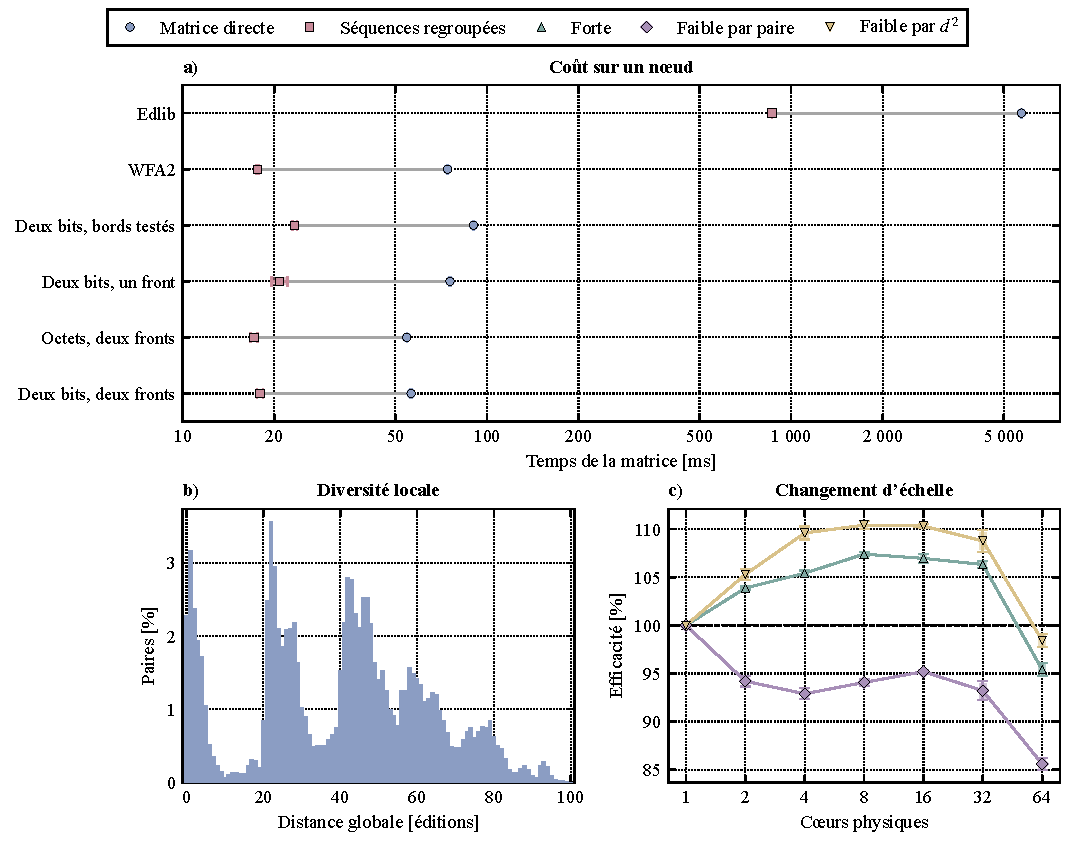
\includegraphics[width=.93\linewidth]{../figures/cpu/cohorte_compacte.pdf}
\caption{Le temps de matrice comprend la préparation et la restitution des scores. La distribution porte sur toutes les paires. Les marques donnent les moyennes de cinq blocs après échauffement, les traits épais leur écart-type et les traits fins l’intervalle à 95\,\%. Pour l’efficacité, l’incertitude du rapport propage celle des deux temps.}\label{fig:cohortecompacte}
\sourcefig{python/studies/cohorte_compacte.py}
\end{figure}
\FloatBarrier
À codage fixé, les sentinelles réduisent le temps moyen de 16,3\,\%. Le parcours bidirectionnel réduit ensuite de 25,5\,\% le temps du front unique. Sur les 8\,128 paires du profil monocœur, le codage en deux bits ramène les défauts L1D de 1092,0 à 266,7 par paire. Les mots compactés occupent 8\,396\,968 octets en plus des séquences originales. La matrice directe prend 54,51~ms en octets et 56,31~ms en deux bits sur 64 cœurs.

La médiane vaut 42 éditions et 11\,954 paires ont la distance nulle. Les 386 séquences distinctes demandent 74\,305 alignements après regroupement. Les 523\,776 scores sont ensuite restitués dans l’ordre des haplotypes. Sur 64 cœurs, cette opération porte les temps totaux à 17,61~ms pour WFA2 et à 17,94~ms pour les deux bits. D’un à 64 cœurs, l’efficacité des fronts compactés atteint 95,4\,\% à matrice fixe et 85,6\,\% à nombre de paires par cœur comparable. La moyenne de \(d^2\) passe de 1\,852,50 à 2\,130,57 entre les deux préfixes. Pondérée par \(d^2\), indicateur du nombre d’états des fronts, l’efficacité faible vaut 98,4\,\%.

\synthese{À 64 cœurs, les fronts compactés calculent la matrice directe en 56,31 \(\pm\) 0,32~ms, contre 74,24 \(\pm\) 0,26~ms pour WFA2. Le rapport des temps moyens vaut 1,32 pour WFA2 et 101,45 pour Edlib.}

\subsection{Construction des arbres de phage}
Le panel réunit la référence du phage \(\phi\)X174 (\texttt{NC\_001422.1}) et 63 autres génomes complets obtenus avec NCBI Datasets~18.41.1~\cite{phixref,ncbidatasets}.\footnote{Le manifeste \reposource{results/ncbi/phix174.tsv} donne l’accession versionnée, la longueur et l’empreinte de chaque séquence.} La reconstruction mesure dans quelle proportion les chemins d'un arbre reproduisent leurs distances globales. Une origine différente sur le génome circulaire peut modifier la distance entre les chaînes déposées. Une même édition observée peut aussi résulter de plusieurs événements évolutifs.

UPGMA, la méthode de classification moyenne de Sokal et Michener~\cite{upgma}, joint les groupes \(U,V\) de distance moyenne minimale et place leur parent à la hauteur \(d(U,V)/2\). Pour un troisième groupe \(W\), la nouvelle distance moyenne est pondérée par les effectifs. Saitou et Nei ont proposé Neighbor-Joining (NJ) pour construire un arbre non enraciné~\cite{nj}. NJ joint la paire qui minimise \(Q_{ij}\), où \(r\) est le nombre de groupes actifs et \(s_i=\sum_k d_{ik}\).
\[
 d(U\cup V,W)=\frac{|U|d(U,W)+|V|d(V,W)}{|U|+|V|},\qquad
 Q_{ij}=(r-2)d_{ij}-s_i-s_j.
\]
Dans NJ, la première branche mesure \(d_{ij}/2+(s_i-s_j)/(2(r-2))\), la seconde complète \(d_{ij}\). À chaque fusion, les deux implémentations examinent toutes les paires actives. Pour \(N\) feuilles, elles utilisent \(O(N^3)\) opérations et \(O(N^2)\) distances stockées.

Les phylogrammes de la figure~\ref{fig:arbres} utilisent la longueur cumulée des branches comme abscisse. La longueur patristique se calcule par \(t_{ij}=\sum_{e\in\operatorname{path}(i,j)}\ell_e\). Le choix du point de dessin initial de NJ laisse ces sommes invariantes.

\begin{figure}[!htbp]\centering
\resizebox{!}{.68\textheight}{\begin{tikzpicture}[x=1mm,y=-1mm,line width=.3pt]
\node[anchor=west,font=\small\bfseries,inner sep=0pt] at (0.000,-6) {a) UPGMA};
\draw[draw=powderBlue!50!black] (5.447,0.000) -- (34.880,0.000);
\draw[draw=powderBlue!50!black] (6.097,3.240) -- (34.880,3.240);
\draw[draw=powderBlue!50!black] (6.543,6.480) -- (34.880,6.480);
\draw[draw=powderBlue!50!black] (15.886,9.720) -- (34.880,9.720);
\draw[draw=powderBlue!50!black] (15.886,12.960) -- (34.880,12.960);
\draw[draw=powderBlue!50!black] (15.886,9.720) -- (15.886,12.960);
\draw[draw=powderBlue!50!black] (7.494,11.340) -- (15.886,11.340);
\draw[draw=powderBlue!50!black] (20.257,16.200) -- (34.880,16.200);
\draw[draw=powderBlue!50!black] (24.704,19.440) -- (34.880,19.440);
\draw[draw=powderBlue!50!black] (26.287,22.680) -- (34.880,22.680);
\draw[draw=powderBlue!50!black] (26.287,25.920) -- (34.880,25.920);
\draw[draw=powderBlue!50!black] (26.287,22.680) -- (26.287,25.920);
\draw[draw=powderBlue!50!black] (24.704,24.300) -- (26.287,24.300);
\draw[draw=powderBlue!50!black] (24.704,19.440) -- (24.704,24.300);
\draw[draw=powderBlue!50!black] (20.257,21.870) -- (24.704,21.870);
\draw[draw=powderBlue!50!black] (20.257,16.200) -- (20.257,21.870);
\draw[draw=powderBlue!50!black] (8.570,19.035) -- (20.257,19.035);
\draw[draw=powderBlue!50!black] (8.752,29.160) -- (34.880,29.160);
\draw[draw=powderBlue!50!black] (9.265,32.400) -- (34.880,32.400);
\draw[draw=powderBlue!50!black] (11.851,35.640) -- (34.880,35.640);
\draw[draw=powderBlue!50!black] (12.207,38.880) -- (34.880,38.880);
\draw[draw=powderBlue!50!black] (12.984,42.120) -- (34.880,42.120);
\draw[draw=powderBlue!50!black] (13.121,45.360) -- (34.880,45.360);
\draw[draw=powderBlue!50!black] (14.356,48.600) -- (34.880,48.600);
\draw[draw=powderBlue!50!black] (14.502,51.840) -- (34.880,51.840);
\draw[draw=powderBlue!50!black] (15.674,55.080) -- (34.880,55.080);
\draw[draw=powderBlue!50!black] (15.900,58.320) -- (34.880,58.320);
\draw[draw=powderBlue!50!black] (15.961,61.560) -- (34.880,61.560);
\draw[draw=powderBlue!50!black] (16.151,64.800) -- (34.880,64.800);
\draw[draw=powderBlue!50!black] (16.903,68.040) -- (34.880,68.040);
\draw[draw=powderBlue!50!black] (18.247,71.280) -- (34.880,71.280);
\draw[draw=powderBlue!50!black] (20.408,74.520) -- (34.880,74.520);
\draw[draw=powderBlue!50!black] (27.945,77.760) -- (34.880,77.760);
\draw[draw=powderBlue!50!black] (32.618,81.000) -- (34.880,81.000);
\draw[draw=powderBlue!50!black] (33.071,84.240) -- (34.880,84.240);
\draw[draw=powderBlue!50!black] (33.071,87.480) -- (34.880,87.480);
\draw[draw=powderBlue!50!black] (33.071,84.240) -- (33.071,87.480);
\draw[draw=powderBlue!50!black] (32.618,85.860) -- (33.071,85.860);
\draw[draw=powderBlue!50!black] (32.618,81.000) -- (32.618,85.860);
\draw[draw=powderBlue!50!black] (27.945,83.430) -- (32.618,83.430);
\draw[draw=powderBlue!50!black] (27.945,77.760) -- (27.945,83.430);
\draw[draw=powderBlue!50!black] (22.001,80.595) -- (27.945,80.595);
\draw[draw=powderBlue!50!black] (27.644,90.720) -- (34.880,90.720);
\draw[draw=powderBlue!50!black] (33.071,93.960) -- (34.880,93.960);
\draw[draw=powderBlue!50!black] (33.071,97.200) -- (34.880,97.200);
\draw[draw=powderBlue!50!black] (33.071,93.960) -- (33.071,97.200);
\draw[draw=powderBlue!50!black] (27.644,95.580) -- (33.071,95.580);
\draw[draw=powderBlue!50!black] (27.644,90.720) -- (27.644,95.580);
\draw[draw=powderBlue!50!black] (23.613,93.150) -- (27.644,93.150);
\draw[draw=powderBlue!50!black] (30.583,100.440) -- (34.880,100.440);
\draw[draw=powderBlue!50!black] (33.523,103.680) -- (34.880,103.680);
\draw[draw=powderBlue!50!black] (33.523,106.920) -- (34.880,106.920);
\draw[draw=powderBlue!50!black] (33.523,103.680) -- (33.523,106.920);
\draw[draw=powderBlue!50!black] (30.583,105.300) -- (33.523,105.300);
\draw[draw=powderBlue!50!black] (30.583,100.440) -- (30.583,105.300);
\draw[draw=powderBlue!50!black] (26.758,102.870) -- (30.583,102.870);
\draw[draw=powderBlue!50!black] (29.212,110.160) -- (34.880,110.160);
\draw[draw=powderBlue!50!black] (32.618,113.400) -- (34.880,113.400);
\draw[draw=powderBlue!50!black] (32.618,116.640) -- (34.880,116.640);
\draw[draw=powderBlue!50!black] (32.618,113.400) -- (32.618,116.640);
\draw[draw=powderBlue!50!black] (30.862,115.020) -- (32.618,115.020);
\draw[draw=powderBlue!50!black] (31.488,119.880) -- (34.880,119.880);
\draw[draw=powderBlue!50!black] (33.674,123.120) -- (34.880,123.120);
\draw[draw=powderBlue!50!black] (33.975,126.360) -- (34.880,126.360);
\draw[draw=powderBlue!50!black] (33.975,129.600) -- (34.880,129.600);
\draw[draw=powderBlue!50!black] (33.975,132.840) -- (34.880,132.840);
\draw[draw=powderBlue!50!black] (33.975,129.600) -- (33.975,132.840);
\draw[draw=powderBlue!50!black] (33.975,131.220) -- (33.975,131.220);
\draw[draw=powderBlue!50!black] (33.975,126.360) -- (33.975,131.220);
\draw[draw=powderBlue!50!black] (33.674,128.790) -- (33.975,128.790);
\draw[draw=powderBlue!50!black] (33.674,123.120) -- (33.674,128.790);
\draw[draw=powderBlue!50!black] (32.505,125.955) -- (33.674,125.955);
\draw[draw=powderBlue!50!black] (33.975,136.080) -- (34.880,136.080);
\draw[draw=powderBlue!50!black] (33.975,139.320) -- (34.880,139.320);
\draw[draw=powderBlue!50!black] (33.975,136.080) -- (33.975,139.320);
\draw[draw=powderBlue!50!black] (33.221,137.700) -- (33.975,137.700);
\draw[draw=powderBlue!50!black] (33.613,142.560) -- (34.880,142.560);
\draw[draw=powderBlue!50!black] (34.880,145.800) -- (34.880,145.800);
\draw[draw=powderBlue!50!black] (34.880,149.040) -- (34.880,149.040);
\draw[draw=powderBlue!50!black] (34.880,145.800) -- (34.880,149.040);
\draw[draw=powderBlue!50!black] (34.126,147.420) -- (34.880,147.420);
\draw[draw=powderBlue!50!black] (34.201,152.280) -- (34.880,152.280);
\draw[draw=powderBlue!50!black] (34.427,155.520) -- (34.880,155.520);
\draw[draw=powderBlue!50!black] (34.427,158.760) -- (34.880,158.760);
\draw[draw=powderBlue!50!black] (34.427,155.520) -- (34.427,158.760);
\draw[draw=powderBlue!50!black] (34.201,157.140) -- (34.427,157.140);
\draw[draw=powderBlue!50!black] (34.201,152.280) -- (34.201,157.140);
\draw[draw=powderBlue!50!black] (34.126,154.710) -- (34.201,154.710);
\draw[draw=powderBlue!50!black] (34.126,147.420) -- (34.126,154.710);
\draw[draw=powderBlue!50!black] (33.613,151.065) -- (34.126,151.065);
\draw[draw=powderBlue!50!black] (33.613,142.560) -- (33.613,151.065);
\draw[draw=powderBlue!50!black] (33.221,146.812) -- (33.613,146.812);
\draw[draw=powderBlue!50!black] (33.221,137.700) -- (33.221,146.812);
\draw[draw=powderBlue!50!black] (32.505,142.256) -- (33.221,142.256);
\draw[draw=powderBlue!50!black] (32.505,125.955) -- (32.505,142.256);
\draw[draw=powderBlue!50!black] (31.488,134.106) -- (32.505,134.106);
\draw[draw=powderBlue!50!black] (31.488,119.880) -- (31.488,134.106);
\draw[draw=powderBlue!50!black] (30.862,126.993) -- (31.488,126.993);
\draw[draw=powderBlue!50!black] (30.862,115.020) -- (30.862,126.993);
\draw[draw=powderBlue!50!black] (29.212,121.006) -- (30.862,121.006);
\draw[draw=powderBlue!50!black] (29.212,110.160) -- (29.212,121.006);
\draw[draw=powderBlue!50!black] (26.758,115.583) -- (29.212,115.583);
\draw[draw=powderBlue!50!black] (26.758,102.870) -- (26.758,115.583);
\draw[draw=powderBlue!50!black] (23.613,109.227) -- (26.758,109.227);
\draw[draw=powderBlue!50!black] (23.613,93.150) -- (23.613,109.227);
\draw[draw=powderBlue!50!black] (22.001,101.188) -- (23.613,101.188);
\draw[draw=powderBlue!50!black] (22.001,80.595) -- (22.001,101.188);
\draw[draw=powderBlue!50!black] (20.408,90.892) -- (22.001,90.892);
\draw[draw=powderBlue!50!black] (20.408,74.520) -- (20.408,90.892);
\draw[draw=powderBlue!50!black] (18.247,82.706) -- (20.408,82.706);
\draw[draw=powderBlue!50!black] (18.247,71.280) -- (18.247,82.706);
\draw[draw=powderBlue!50!black] (16.903,76.993) -- (18.247,76.993);
\draw[draw=powderBlue!50!black] (16.903,68.040) -- (16.903,76.993);
\draw[draw=powderBlue!50!black] (16.151,72.516) -- (16.903,72.516);
\draw[draw=powderBlue!50!black] (16.151,64.800) -- (16.151,72.516);
\draw[draw=powderBlue!50!black] (15.961,68.658) -- (16.151,68.658);
\draw[draw=powderBlue!50!black] (15.961,61.560) -- (15.961,68.658);
\draw[draw=powderBlue!50!black] (15.900,65.109) -- (15.961,65.109);
\draw[draw=powderBlue!50!black] (15.900,58.320) -- (15.900,65.109);
\draw[draw=powderBlue!50!black] (15.674,61.715) -- (15.900,61.715);
\draw[draw=powderBlue!50!black] (15.674,55.080) -- (15.674,61.715);
\draw[draw=powderBlue!50!black] (14.502,58.397) -- (15.674,58.397);
\draw[draw=powderBlue!50!black] (14.502,51.840) -- (14.502,58.397);
\draw[draw=powderBlue!50!black] (14.356,55.119) -- (14.502,55.119);
\draw[draw=powderBlue!50!black] (14.356,48.600) -- (14.356,55.119);
\draw[draw=powderBlue!50!black] (13.121,51.859) -- (14.356,51.859);
\draw[draw=powderBlue!50!black] (13.121,45.360) -- (13.121,51.859);
\draw[draw=powderBlue!50!black] (12.984,48.610) -- (13.121,48.610);
\draw[draw=powderBlue!50!black] (12.984,42.120) -- (12.984,48.610);
\draw[draw=powderBlue!50!black] (12.207,45.365) -- (12.984,45.365);
\draw[draw=powderBlue!50!black] (12.207,38.880) -- (12.207,45.365);
\draw[draw=powderBlue!50!black] (11.851,42.122) -- (12.207,42.122);
\draw[draw=powderBlue!50!black] (11.851,35.640) -- (11.851,42.122);
\draw[draw=powderBlue!50!black] (9.265,38.881) -- (11.851,38.881);
\draw[draw=powderBlue!50!black] (9.265,32.400) -- (9.265,38.881);
\draw[draw=powderBlue!50!black] (8.752,35.641) -- (9.265,35.641);
\draw[draw=powderBlue!50!black] (8.752,29.160) -- (8.752,35.641);
\draw[draw=powderBlue!50!black] (8.570,32.400) -- (8.752,32.400);
\draw[draw=powderBlue!50!black] (8.570,19.035) -- (8.570,32.400);
\draw[draw=powderBlue!50!black] (7.494,25.718) -- (8.570,25.718);
\draw[draw=powderBlue!50!black] (7.494,11.340) -- (7.494,25.718);
\draw[draw=powderBlue!50!black] (6.543,18.529) -- (7.494,18.529);
\draw[draw=powderBlue!50!black] (6.543,6.480) -- (6.543,18.529);
\draw[draw=powderBlue!50!black] (6.097,12.504) -- (6.543,12.504);
\draw[draw=powderBlue!50!black] (6.097,3.240) -- (6.097,12.504);
\draw[draw=powderBlue!50!black] (5.447,7.872) -- (6.097,7.872);
\draw[draw=powderBlue!50!black] (5.447,0.000) -- (5.447,7.872);
\draw[draw=powderBlue!50!black] (0.000,3.936) -- (5.447,3.936);
\draw[draw=powderBlue!50!black] (16.338,162.000) -- (34.880,162.000);
\draw[draw=powderBlue!50!black] (31.714,165.240) -- (34.880,165.240);
\draw[draw=powderBlue!50!black] (31.714,168.480) -- (34.880,168.480);
\draw[draw=powderBlue!50!black] (31.714,165.240) -- (31.714,168.480);
\draw[draw=powderBlue!50!black] (16.338,166.860) -- (31.714,166.860);
\draw[draw=powderBlue!50!black] (16.338,162.000) -- (16.338,166.860);
\draw[draw=powderBlue!50!black] (0.976,164.430) -- (16.338,164.430);
\draw[draw=powderBlue!50!black] (24.704,171.720) -- (34.880,171.720);
\draw[draw=powderBlue!50!black] (31.714,174.960) -- (34.880,174.960);
\draw[draw=powderBlue!50!black] (31.714,178.200) -- (34.880,178.200);
\draw[draw=powderBlue!50!black] (31.714,174.960) -- (31.714,178.200);
\draw[draw=powderBlue!50!black] (24.704,176.580) -- (31.714,176.580);
\draw[draw=powderBlue!50!black] (24.704,171.720) -- (24.704,176.580);
\draw[draw=powderBlue!50!black] (11.797,174.150) -- (24.704,174.150);
\draw[draw=powderBlue!50!black] (31.262,181.440) -- (34.880,181.440);
\draw[draw=powderBlue!50!black] (32.166,184.680) -- (34.880,184.680);
\draw[draw=powderBlue!50!black] (32.166,187.920) -- (34.880,187.920);
\draw[draw=powderBlue!50!black] (32.166,184.680) -- (32.166,187.920);
\draw[draw=powderBlue!50!black] (31.262,186.300) -- (32.166,186.300);
\draw[draw=powderBlue!50!black] (31.262,181.440) -- (31.262,186.300);
\draw[draw=powderBlue!50!black] (16.278,183.870) -- (31.262,183.870);
\draw[draw=powderBlue!50!black] (22.217,191.160) -- (34.880,191.160);
\draw[draw=powderBlue!50!black] (28.850,194.400) -- (34.880,194.400);
\draw[draw=powderBlue!50!black] (29.679,197.640) -- (34.880,197.640);
\draw[draw=powderBlue!50!black] (31.714,200.880) -- (34.880,200.880);
\draw[draw=powderBlue!50!black] (31.714,204.120) -- (34.880,204.120);
\draw[draw=powderBlue!50!black] (31.714,200.880) -- (31.714,204.120);
\draw[draw=powderBlue!50!black] (29.679,202.500) -- (31.714,202.500);
\draw[draw=powderBlue!50!black] (29.679,197.640) -- (29.679,202.500);
\draw[draw=powderBlue!50!black] (28.850,200.070) -- (29.679,200.070);
\draw[draw=powderBlue!50!black] (28.850,194.400) -- (28.850,200.070);
\draw[draw=powderBlue!50!black] (22.217,197.235) -- (28.850,197.235);
\draw[draw=powderBlue!50!black] (22.217,191.160) -- (22.217,197.235);
\draw[draw=powderBlue!50!black] (16.278,194.198) -- (22.217,194.198);
\draw[draw=powderBlue!50!black] (16.278,183.870) -- (16.278,194.198);
\draw[draw=powderBlue!50!black] (11.797,189.034) -- (16.278,189.034);
\draw[draw=powderBlue!50!black] (11.797,174.150) -- (11.797,189.034);
\draw[draw=powderBlue!50!black] (0.976,181.592) -- (11.797,181.592);
\draw[draw=powderBlue!50!black] (0.976,164.430) -- (0.976,181.592);
\draw[draw=powderBlue!50!black] (0.000,173.011) -- (0.976,173.011);
\draw[draw=powderBlue!50!black] (0.000,3.936) -- (0.000,173.011);
\draw[densely dotted,black!36] (34.880,0.000) -- (35.880,0.000);
\node[anchor=west,inner sep=0pt,font=\rmfamily\fontsize{7}{7}\selectfont] at (36.880,0.000) {EF380022.1};
\draw[densely dotted,black!36] (34.880,3.240) -- (35.880,3.240);
\node[anchor=west,inner sep=0pt,font=\rmfamily\fontsize{7}{7}\selectfont] at (36.880,3.240) {EF380026.1};
\draw[densely dotted,black!36] (34.880,6.480) -- (35.880,6.480);
\node[anchor=west,inner sep=0pt,font=\rmfamily\fontsize{7}{7}\selectfont] at (36.880,6.480) {EF380023.1};
\draw[densely dotted,black!36] (34.880,9.720) -- (35.880,9.720);
\node[anchor=west,inner sep=0pt,font=\rmfamily\fontsize{7}{7}\selectfont] at (36.880,9.720) {EF380024.1};
\draw[densely dotted,black!36] (34.880,12.960) -- (35.880,12.960);
\node[anchor=west,inner sep=0pt,font=\rmfamily\fontsize{7}{7}\selectfont] at (36.880,12.960) {EF380025.1};
\draw[densely dotted,black!36] (34.880,16.200) -- (35.880,16.200);
\node[anchor=west,inner sep=0pt,font=\rmfamily\fontsize{7}{7}\selectfont] at (36.880,16.200) {EF380029.1};
\draw[densely dotted,black!36] (34.880,19.440) -- (35.880,19.440);
\node[anchor=west,inner sep=0pt,font=\rmfamily\fontsize{7}{7}\selectfont] at (36.880,19.440) {EF380021.1};
\draw[densely dotted,black!36] (34.880,22.680) -- (35.880,22.680);
\node[anchor=west,inner sep=0pt,font=\rmfamily\fontsize{7}{7}\selectfont] at (36.880,22.680) {EF380028.1};
\draw[densely dotted,black!36] (34.880,25.920) -- (35.880,25.920);
\node[anchor=west,inner sep=0pt,font=\rmfamily\fontsize{7}{7}\selectfont] at (36.880,25.920) {EF380030.1};
\draw[densely dotted,black!36] (34.880,29.160) -- (35.880,29.160);
\node[anchor=west,inner sep=0pt,font=\rmfamily\fontsize{7}{7}\selectfont] at (36.880,29.160) {EF380027.1};
\draw[densely dotted,black!36] (34.880,32.400) -- (35.880,32.400);
\node[anchor=west,inner sep=0pt,font=\rmfamily\fontsize{7}{7}\selectfont] at (36.880,32.400) {EF380012.1};
\draw[densely dotted,black!36] (34.880,35.640) -- (35.880,35.640);
\node[anchor=west,inner sep=0pt,font=\rmfamily\fontsize{7}{7}\selectfont] at (36.880,35.640) {EF380013.1};
\draw[densely dotted,black!36] (34.880,38.880) -- (35.880,38.880);
\node[anchor=west,inner sep=0pt,font=\rmfamily\fontsize{7}{7}\selectfont] at (36.880,38.880) {EF380011.1};
\draw[densely dotted,black!36] (34.880,42.120) -- (35.880,42.120);
\node[anchor=west,inner sep=0pt,font=\rmfamily\fontsize{7}{7}\selectfont] at (36.880,42.120) {EF380014.1};
\draw[densely dotted,black!36] (34.880,45.360) -- (35.880,45.360);
\node[anchor=west,inner sep=0pt,font=\rmfamily\fontsize{7}{7}\selectfont] at (36.880,45.360) {EF380018.1};
\draw[densely dotted,black!36] (34.880,48.600) -- (35.880,48.600);
\node[anchor=west,inner sep=0pt,font=\rmfamily\fontsize{7}{7}\selectfont] at (36.880,48.600) {GQ153914.1};
\draw[densely dotted,black!36] (34.880,51.840) -- (35.880,51.840);
\node[anchor=west,inner sep=0pt,font=\rmfamily\fontsize{7}{7}\selectfont] at (36.880,51.840) {GQ153913.1};
\draw[densely dotted,black!36] (34.880,55.080) -- (35.880,55.080);
\node[anchor=west,inner sep=0pt,font=\rmfamily\fontsize{7}{7}\selectfont] at (36.880,55.080) {EF380010.1};
\draw[densely dotted,black!36] (34.880,58.320) -- (35.880,58.320);
\node[anchor=west,inner sep=0pt,font=\rmfamily\fontsize{7}{7}\selectfont] at (36.880,58.320) {EF380016.1};
\draw[densely dotted,black!36] (34.880,61.560) -- (35.880,61.560);
\node[anchor=west,inner sep=0pt,font=\rmfamily\fontsize{7}{7}\selectfont] at (36.880,61.560) {EF380019.1};
\draw[densely dotted,black!36] (34.880,64.800) -- (35.880,64.800);
\node[anchor=west,inner sep=0pt,font=\rmfamily\fontsize{7}{7}\selectfont] at (36.880,64.800) {EF380020.1};
\draw[densely dotted,black!36] (34.880,68.040) -- (35.880,68.040);
\node[anchor=west,inner sep=0pt,font=\rmfamily\fontsize{7}{7}\selectfont] at (36.880,68.040) {EF380015.1};
\draw[densely dotted,black!36] (34.880,71.280) -- (35.880,71.280);
\node[anchor=west,inner sep=0pt,font=\rmfamily\fontsize{7}{7}\selectfont] at (36.880,71.280) {EF380017.1};
\draw[densely dotted,black!36] (34.880,74.520) -- (35.880,74.520);
\node[anchor=west,inner sep=0pt,font=\rmfamily\fontsize{7}{7}\selectfont] at (36.880,74.520) {GQ153912.1};
\draw[densely dotted,black!36] (34.880,77.760) -- (35.880,77.760);
\node[anchor=west,inner sep=0pt,font=\rmfamily\fontsize{7}{7}\selectfont] at (36.880,77.760) {AF176027.1};
\draw[densely dotted,black!36] (34.880,81.000) -- (35.880,81.000);
\node[anchor=west,inner sep=0pt,font=\rmfamily\fontsize{7}{7}\selectfont] at (36.880,81.000) {AF176033.1};
\draw[densely dotted,black!36] (34.880,84.240) -- (35.880,84.240);
\node[anchor=west,inner sep=0pt,font=\rmfamily\fontsize{7}{7}\selectfont] at (36.880,84.240) {AF176029.1};
\draw[densely dotted,black!36] (34.880,87.480) -- (35.880,87.480);
\node[anchor=west,inner sep=0pt,font=\rmfamily\fontsize{7}{7}\selectfont] at (36.880,87.480) {AF176031.1};
\draw[densely dotted,black!36] (34.880,90.720) -- (35.880,90.720);
\node[anchor=west,inner sep=0pt,font=\rmfamily\fontsize{7}{7}\selectfont] at (36.880,90.720) {AF299313.1};
\draw[densely dotted,black!36] (34.880,93.960) -- (35.880,93.960);
\node[anchor=west,inner sep=0pt,font=\rmfamily\fontsize{7}{7}\selectfont] at (36.880,93.960) {AF299301.1};
\draw[densely dotted,black!36] (34.880,97.200) -- (35.880,97.200);
\node[anchor=west,inner sep=0pt,font=\rmfamily\fontsize{7}{7}\selectfont] at (36.880,97.200) {AF299305.1};
\draw[densely dotted,black!36] (34.880,100.440) -- (35.880,100.440);
\node[anchor=west,inner sep=0pt,font=\rmfamily\fontsize{7}{7}\selectfont] at (36.880,100.440) {EF380009.1};
\draw[densely dotted,black!36] (34.880,103.680) -- (35.880,103.680);
\node[anchor=west,inner sep=0pt,font=\rmfamily\fontsize{7}{7}\selectfont] at (36.880,103.680) {EF380031.1};
\draw[densely dotted,black!36] (34.880,106.920) -- (35.880,106.920);
\node[anchor=west,inner sep=0pt,font=\rmfamily\fontsize{7}{7}\selectfont] at (36.880,106.920) {EF380032.1};
\draw[densely dotted,black!36] (34.880,110.160) -- (35.880,110.160);
\node[anchor=west,inner sep=0pt,font=\rmfamily\fontsize{7}{7}\selectfont] at (36.880,110.160) {GQ153915.1};
\draw[densely dotted,black!36] (34.880,113.400) -- (35.880,113.400);
\node[anchor=west,inner sep=0pt,font=\rmfamily\fontsize{7}{7}\selectfont] at (36.880,113.400) {NC\_001422.1};
\draw[densely dotted,black!36] (34.880,116.640) -- (35.880,116.640);
\node[anchor=west,inner sep=0pt,font=\rmfamily\fontsize{7}{7}\selectfont] at (36.880,116.640) {CP004084.1};
\draw[densely dotted,black!36] (34.880,119.880) -- (35.880,119.880);
\node[anchor=west,inner sep=0pt,font=\rmfamily\fontsize{7}{7}\selectfont] at (36.880,119.880) {AF299302.1};
\draw[densely dotted,black!36] (34.880,123.120) -- (35.880,123.120);
\node[anchor=west,inner sep=0pt,font=\rmfamily\fontsize{7}{7}\selectfont] at (36.880,123.120) {HM753662.1};
\draw[densely dotted,black!36] (34.880,126.360) -- (35.880,126.360);
\node[anchor=west,inner sep=0pt,font=\rmfamily\fontsize{7}{7}\selectfont] at (36.880,126.360) {GU385905.1};
\draw[densely dotted,black!36] (34.880,129.600) -- (35.880,129.600);
\node[anchor=west,inner sep=0pt,font=\rmfamily\fontsize{7}{7}\selectfont] at (36.880,129.600) {AF176034.1};
\draw[densely dotted,black!36] (34.880,132.840) -- (35.880,132.840);
\node[anchor=west,inner sep=0pt,font=\rmfamily\fontsize{7}{7}\selectfont] at (36.880,132.840) {FJ849058.1};
\draw[densely dotted,black!36] (34.880,136.080) -- (35.880,136.080);
\node[anchor=west,inner sep=0pt,font=\rmfamily\fontsize{7}{7}\selectfont] at (36.880,136.080) {HM753664.1};
\draw[densely dotted,black!36] (34.880,139.320) -- (35.880,139.320);
\node[anchor=west,inner sep=0pt,font=\rmfamily\fontsize{7}{7}\selectfont] at (36.880,139.320) {HM753665.1};
\draw[densely dotted,black!36] (34.880,142.560) -- (35.880,142.560);
\node[anchor=west,inner sep=0pt,font=\rmfamily\fontsize{7}{7}\selectfont] at (36.880,142.560) {HM753658.1};
\draw[densely dotted,black!36] (34.880,145.800) -- (35.880,145.800);
\node[anchor=west,inner sep=0pt,font=\rmfamily\fontsize{7}{7}\selectfont] at (36.880,145.800) {HM753660.1};
\draw[densely dotted,black!36] (34.880,149.040) -- (35.880,149.040);
\node[anchor=west,inner sep=0pt,font=\rmfamily\fontsize{7}{7}\selectfont] at (36.880,149.040) {HM753661.1};
\draw[densely dotted,black!36] (34.880,152.280) -- (35.880,152.280);
\node[anchor=west,inner sep=0pt,font=\rmfamily\fontsize{7}{7}\selectfont] at (36.880,152.280) {HM753666.1};
\draw[densely dotted,black!36] (34.880,155.520) -- (35.880,155.520);
\node[anchor=west,inner sep=0pt,font=\rmfamily\fontsize{7}{7}\selectfont] at (36.880,155.520) {HM753659.1};
\draw[densely dotted,black!36] (34.880,158.760) -- (35.880,158.760);
\node[anchor=west,inner sep=0pt,font=\rmfamily\fontsize{7}{7}\selectfont] at (36.880,158.760) {HM753663.1};
\draw[densely dotted,black!36] (34.880,162.000) -- (35.880,162.000);
\node[anchor=west,inner sep=0pt,font=\rmfamily\fontsize{7}{7}\selectfont] at (36.880,162.000) {AF299307.1};
\draw[densely dotted,black!36] (34.880,165.240) -- (35.880,165.240);
\node[anchor=west,inner sep=0pt,font=\rmfamily\fontsize{7}{7}\selectfont] at (36.880,165.240) {AF299306.1};
\draw[densely dotted,black!36] (34.880,168.480) -- (35.880,168.480);
\node[anchor=west,inner sep=0pt,font=\rmfamily\fontsize{7}{7}\selectfont] at (36.880,168.480) {AF299308.1};
\draw[densely dotted,black!36] (34.880,171.720) -- (35.880,171.720);
\node[anchor=west,inner sep=0pt,font=\rmfamily\fontsize{7}{7}\selectfont] at (36.880,171.720) {AF299312.1};
\draw[densely dotted,black!36] (34.880,174.960) -- (35.880,174.960);
\node[anchor=west,inner sep=0pt,font=\rmfamily\fontsize{7}{7}\selectfont] at (36.880,174.960) {AF299303.1};
\draw[densely dotted,black!36] (34.880,178.200) -- (35.880,178.200);
\node[anchor=west,inner sep=0pt,font=\rmfamily\fontsize{7}{7}\selectfont] at (36.880,178.200) {AF299311.1};
\draw[densely dotted,black!36] (34.880,181.440) -- (35.880,181.440);
\node[anchor=west,inner sep=0pt,font=\rmfamily\fontsize{7}{7}\selectfont] at (36.880,181.440) {AF176032.1};
\draw[densely dotted,black!36] (34.880,184.680) -- (35.880,184.680);
\node[anchor=west,inner sep=0pt,font=\rmfamily\fontsize{7}{7}\selectfont] at (36.880,184.680) {AF176028.1};
\draw[densely dotted,black!36] (34.880,187.920) -- (35.880,187.920);
\node[anchor=west,inner sep=0pt,font=\rmfamily\fontsize{7}{7}\selectfont] at (36.880,187.920) {AF176030.1};
\draw[densely dotted,black!36] (34.880,191.160) -- (35.880,191.160);
\node[anchor=west,inner sep=0pt,font=\rmfamily\fontsize{7}{7}\selectfont] at (36.880,191.160) {AF299314.1};
\draw[densely dotted,black!36] (34.880,194.400) -- (35.880,194.400);
\node[anchor=west,inner sep=0pt,font=\rmfamily\fontsize{7}{7}\selectfont] at (36.880,194.400) {AF299309.1};
\draw[densely dotted,black!36] (34.880,197.640) -- (35.880,197.640);
\node[anchor=west,inner sep=0pt,font=\rmfamily\fontsize{7}{7}\selectfont] at (36.880,197.640) {AF299310.1};
\draw[densely dotted,black!36] (34.880,200.880) -- (35.880,200.880);
\node[anchor=west,inner sep=0pt,font=\rmfamily\fontsize{7}{7}\selectfont] at (36.880,200.880) {AF299300.1};
\draw[densely dotted,black!36] (34.880,204.120) -- (35.880,204.120);
\node[anchor=west,inner sep=0pt,font=\rmfamily\fontsize{7}{7}\selectfont] at (36.880,204.120) {AF299304.1};
\draw[line width=.6pt] (0.000,210) -- ++(9.045,0) node[midway,below=2pt,font=\scriptsize] {10 éditions};
\node[anchor=west,font=\small\bfseries,inner sep=0pt] at (62.880,-6) {b) Neighbor-Joining};
\draw[draw=powderTeal!50!black] (62.887,0.000) -- (62.887,0.000);
\draw[draw=powderTeal!50!black] (62.887,3.240) -- (63.791,3.240);
\draw[draw=powderTeal!50!black] (62.887,0.000) -- (62.887,3.240);
\draw[draw=powderTeal!50!black] (62.880,1.620) -- (62.887,1.620);
\draw[draw=powderTeal!50!black] (63.777,6.480) -- (63.792,6.480);
\draw[draw=powderTeal!50!black] (64.666,9.720) -- (65.571,9.720);
\draw[draw=powderTeal!50!black] (64.666,12.960) -- (65.571,12.960);
\draw[draw=powderTeal!50!black] (64.666,9.720) -- (64.666,12.960);
\draw[draw=powderTeal!50!black] (63.777,11.340) -- (64.666,11.340);
\draw[draw=powderTeal!50!black] (63.777,6.480) -- (63.777,11.340);
\draw[draw=powderTeal!50!black] (62.887,8.910) -- (63.777,8.910);
\draw[draw=powderTeal!50!black] (62.904,16.200) -- (64.691,16.200);
\draw[draw=powderTeal!50!black] (64.603,19.440) -- (65.372,19.440);
\draw[draw=powderTeal!50!black] (75.779,22.680) -- (78.780,22.680);
\draw[draw=powderTeal!50!black] (84.536,25.920) -- (85.554,25.920);
\draw[draw=powderTeal!50!black] (85.327,29.160) -- (86.952,29.160);
\draw[draw=powderTeal!50!black] (85.327,32.400) -- (88.225,32.400);
\draw[draw=powderTeal!50!black] (85.327,29.160) -- (85.327,32.400);
\draw[draw=powderTeal!50!black] (84.536,30.780) -- (85.327,30.780);
\draw[draw=powderTeal!50!black] (84.536,25.920) -- (84.536,30.780);
\draw[draw=powderTeal!50!black] (75.779,28.350) -- (84.536,28.350);
\draw[draw=powderTeal!50!black] (75.779,22.680) -- (75.779,28.350);
\draw[draw=powderTeal!50!black] (69.377,25.515) -- (75.779,25.515);
\draw[draw=powderTeal!50!black] (113.436,35.640) -- (114.751,35.640);
\draw[draw=powderTeal!50!black] (114.835,38.880) -- (117.586,38.880);
\draw[draw=powderTeal!50!black] (114.835,42.120) -- (119.320,42.120);
\draw[draw=powderTeal!50!black] (114.835,38.880) -- (114.835,42.120);
\draw[draw=powderTeal!50!black] (113.436,40.500) -- (114.835,40.500);
\draw[draw=powderTeal!50!black] (113.436,35.640) -- (113.436,40.500);
\draw[draw=powderTeal!50!black] (92.589,38.070) -- (113.436,38.070);
\draw[draw=powderTeal!50!black] (95.894,45.360) -- (109.861,45.360);
\draw[draw=powderTeal!50!black] (106.473,48.600) -- (130.888,48.600);
\draw[draw=powderTeal!50!black] (119.142,51.840) -- (120.402,51.840);
\draw[draw=powderTeal!50!black] (120.595,55.080) -- (125.992,55.080);
\draw[draw=powderTeal!50!black] (120.595,58.320) -- (136.000,58.320);
\draw[draw=powderTeal!50!black] (120.595,55.080) -- (120.595,58.320);
\draw[draw=powderTeal!50!black] (119.142,56.700) -- (120.595,56.700);
\draw[draw=powderTeal!50!black] (119.142,51.840) -- (119.142,56.700);
\draw[draw=powderTeal!50!black] (106.473,54.270) -- (119.142,54.270);
\draw[draw=powderTeal!50!black] (106.473,48.600) -- (106.473,54.270);
\draw[draw=powderTeal!50!black] (96.681,51.435) -- (106.473,51.435);
\draw[draw=powderTeal!50!black] (99.213,61.560) -- (100.225,61.560);
\draw[draw=powderTeal!50!black] (104.532,64.800) -- (104.768,64.800);
\draw[draw=powderTeal!50!black] (105.200,68.040) -- (112.521,68.040);
\draw[draw=powderTeal!50!black] (105.200,71.280) -- (111.447,71.280);
\draw[draw=powderTeal!50!black] (105.200,68.040) -- (105.200,71.280);
\draw[draw=powderTeal!50!black] (104.532,69.660) -- (105.200,69.660);
\draw[draw=powderTeal!50!black] (104.532,64.800) -- (104.532,69.660);
\draw[draw=powderTeal!50!black] (99.213,67.230) -- (104.532,67.230);
\draw[draw=powderTeal!50!black] (99.213,61.560) -- (99.213,67.230);
\draw[draw=powderTeal!50!black] (96.681,64.395) -- (99.213,64.395);
\draw[draw=powderTeal!50!black] (96.681,51.435) -- (96.681,64.395);
\draw[draw=powderTeal!50!black] (95.894,57.915) -- (96.681,57.915);
\draw[draw=powderTeal!50!black] (95.894,45.360) -- (95.894,57.915);
\draw[draw=powderTeal!50!black] (92.589,51.638) -- (95.894,51.638);
\draw[draw=powderTeal!50!black] (92.589,38.070) -- (92.589,51.638);
\draw[draw=powderTeal!50!black] (71.782,44.854) -- (92.589,44.854);
\draw[draw=powderTeal!50!black] (81.948,74.520) -- (91.095,74.520);
\draw[draw=powderTeal!50!black] (104.004,77.760) -- (104.106,77.760);
\draw[draw=powderTeal!50!black] (104.004,81.000) -- (110.234,81.000);
\draw[draw=powderTeal!50!black] (104.004,77.760) -- (104.004,81.000);
\draw[draw=powderTeal!50!black] (81.948,79.380) -- (104.004,79.380);
\draw[draw=powderTeal!50!black] (81.948,74.520) -- (81.948,79.380);
\draw[draw=powderTeal!50!black] (77.017,76.950) -- (81.948,76.950);
\draw[draw=powderTeal!50!black] (78.079,84.240) -- (78.155,84.240);
\draw[draw=powderTeal!50!black] (78.079,87.480) -- (81.620,87.480);
\draw[draw=powderTeal!50!black] (78.079,84.240) -- (78.079,87.480);
\draw[draw=powderTeal!50!black] (77.017,85.860) -- (78.079,85.860);
\draw[draw=powderTeal!50!black] (77.017,76.950) -- (77.017,85.860);
\draw[draw=powderTeal!50!black] (71.782,81.405) -- (77.017,81.405);
\draw[draw=powderTeal!50!black] (71.782,44.854) -- (71.782,81.405);
\draw[draw=powderTeal!50!black] (69.377,63.129) -- (71.782,63.129);
\draw[draw=powderTeal!50!black] (69.377,25.515) -- (69.377,63.129);
\draw[draw=powderTeal!50!black] (67.071,44.322) -- (69.377,44.322);
\draw[draw=powderTeal!50!black] (67.390,90.720) -- (69.264,90.720);
\draw[draw=powderTeal!50!black] (73.658,93.960) -- (73.752,93.960);
\draw[draw=powderTeal!50!black] (74.242,97.200) -- (95.196,97.200);
\draw[draw=powderTeal!50!black] (74.995,100.440) -- (87.119,100.440);
\draw[draw=powderTeal!50!black] (74.995,103.680) -- (95.432,103.680);
\draw[draw=powderTeal!50!black] (74.995,100.440) -- (74.995,103.680);
\draw[draw=powderTeal!50!black] (74.242,102.060) -- (74.995,102.060);
\draw[draw=powderTeal!50!black] (74.242,97.200) -- (74.242,102.060);
\draw[draw=powderTeal!50!black] (73.658,99.630) -- (74.242,99.630);
\draw[draw=powderTeal!50!black] (73.658,93.960) -- (73.658,99.630);
\draw[draw=powderTeal!50!black] (67.390,96.795) -- (73.658,96.795);
\draw[draw=powderTeal!50!black] (67.390,90.720) -- (67.390,96.795);
\draw[draw=powderTeal!50!black] (67.071,93.757) -- (67.390,93.757);
\draw[draw=powderTeal!50!black] (67.071,44.322) -- (67.071,93.757);
\draw[draw=powderTeal!50!black] (65.434,69.040) -- (67.071,69.040);
\draw[draw=powderTeal!50!black] (65.682,106.920) -- (65.845,106.920);
\draw[draw=powderTeal!50!black] (66.007,110.160) -- (67.078,110.160);
\draw[draw=powderTeal!50!black] (66.617,113.400) -- (67.541,113.400);
\draw[draw=powderTeal!50!black] (72.290,116.640) -- (73.039,116.640);
\draw[draw=powderTeal!50!black] (89.214,119.880) -- (105.073,119.880);
\draw[draw=powderTeal!50!black] (89.214,123.120) -- (111.343,123.120);
\draw[draw=powderTeal!50!black] (89.214,119.880) -- (89.214,123.120);
\draw[draw=powderTeal!50!black] (73.589,121.500) -- (89.214,121.500);
\draw[draw=powderTeal!50!black] (76.149,126.360) -- (96.536,126.360);
\draw[draw=powderTeal!50!black] (78.691,129.600) -- (96.047,129.600);
\draw[draw=powderTeal!50!black] (92.088,132.840) -- (94.326,132.840);
\draw[draw=powderTeal!50!black] (99.798,136.080) -- (118.515,136.080);
\draw[draw=powderTeal!50!black] (101.885,139.320) -- (110.257,139.320);
\draw[draw=powderTeal!50!black] (101.885,142.560) -- (110.698,142.560);
\draw[draw=powderTeal!50!black] (101.885,139.320) -- (101.885,142.560);
\draw[draw=powderTeal!50!black] (99.798,140.940) -- (101.885,140.940);
\draw[draw=powderTeal!50!black] (99.798,136.080) -- (99.798,140.940);
\draw[draw=powderTeal!50!black] (92.088,138.510) -- (99.798,138.510);
\draw[draw=powderTeal!50!black] (92.088,132.840) -- (92.088,138.510);
\draw[draw=powderTeal!50!black] (78.691,135.675) -- (92.088,135.675);
\draw[draw=powderTeal!50!black] (78.691,129.600) -- (78.691,135.675);
\draw[draw=powderTeal!50!black] (77.525,132.638) -- (78.691,132.638);
\draw[draw=powderTeal!50!black] (78.055,145.800) -- (100.571,145.800);
\draw[draw=powderTeal!50!black] (78.055,149.040) -- (100.762,149.040);
\draw[draw=powderTeal!50!black] (78.055,145.800) -- (78.055,149.040);
\draw[draw=powderTeal!50!black] (77.525,147.420) -- (78.055,147.420);
\draw[draw=powderTeal!50!black] (77.525,132.638) -- (77.525,147.420);
\draw[draw=powderTeal!50!black] (76.149,140.029) -- (77.525,140.029);
\draw[draw=powderTeal!50!black] (76.149,126.360) -- (76.149,140.029);
\draw[draw=powderTeal!50!black] (75.229,133.194) -- (76.149,133.194);
\draw[draw=powderTeal!50!black] (75.246,152.280) -- (94.723,152.280);
\draw[draw=powderTeal!50!black] (76.566,155.520) -- (96.476,155.520);
\draw[draw=powderTeal!50!black] (76.566,158.760) -- (96.453,158.760);
\draw[draw=powderTeal!50!black] (76.566,155.520) -- (76.566,158.760);
\draw[draw=powderTeal!50!black] (75.493,157.140) -- (76.566,157.140);
\draw[draw=powderTeal!50!black] (77.460,162.000) -- (102.542,162.000);
\draw[draw=powderTeal!50!black] (77.460,165.240) -- (92.175,165.240);
\draw[draw=powderTeal!50!black] (77.460,162.000) -- (77.460,165.240);
\draw[draw=powderTeal!50!black] (75.911,163.620) -- (77.460,163.620);
\draw[draw=powderTeal!50!black] (80.957,168.480) -- (113.848,168.480);
\draw[draw=powderTeal!50!black] (81.530,171.720) -- (112.307,171.720);
\draw[draw=powderTeal!50!black] (82.410,174.960) -- (111.363,174.960);
\draw[draw=powderTeal!50!black] (82.410,178.200) -- (108.630,178.200);
\draw[draw=powderTeal!50!black] (82.410,174.960) -- (82.410,178.200);
\draw[draw=powderTeal!50!black] (81.530,176.580) -- (82.410,176.580);
\draw[draw=powderTeal!50!black] (81.530,171.720) -- (81.530,176.580);
\draw[draw=powderTeal!50!black] (80.957,174.150) -- (81.530,174.150);
\draw[draw=powderTeal!50!black] (80.957,168.480) -- (80.957,174.150);
\draw[draw=powderTeal!50!black] (79.830,171.315) -- (80.957,171.315);
\draw[draw=powderTeal!50!black] (80.513,181.440) -- (82.312,181.440);
\draw[draw=powderTeal!50!black] (80.513,184.680) -- (81.427,184.680);
\draw[draw=powderTeal!50!black] (80.513,181.440) -- (80.513,184.680);
\draw[draw=powderTeal!50!black] (79.830,183.060) -- (80.513,183.060);
\draw[draw=powderTeal!50!black] (79.830,171.315) -- (79.830,183.060);
\draw[draw=powderTeal!50!black] (76.963,177.188) -- (79.830,177.188);
\draw[draw=powderTeal!50!black] (78.221,187.920) -- (102.157,187.920);
\draw[draw=powderTeal!50!black] (78.221,191.160) -- (107.649,191.160);
\draw[draw=powderTeal!50!black] (78.221,187.920) -- (78.221,191.160);
\draw[draw=powderTeal!50!black] (76.963,189.540) -- (78.221,189.540);
\draw[draw=powderTeal!50!black] (76.963,177.188) -- (76.963,189.540);
\draw[draw=powderTeal!50!black] (75.911,183.364) -- (76.963,183.364);
\draw[draw=powderTeal!50!black] (75.911,163.620) -- (75.911,183.364);
\draw[draw=powderTeal!50!black] (75.493,173.492) -- (75.911,173.492);
\draw[draw=powderTeal!50!black] (75.493,157.140) -- (75.493,173.492);
\draw[draw=powderTeal!50!black] (75.246,165.316) -- (75.493,165.316);
\draw[draw=powderTeal!50!black] (75.246,152.280) -- (75.246,165.316);
\draw[draw=powderTeal!50!black] (75.229,158.798) -- (75.246,158.798);
\draw[draw=powderTeal!50!black] (75.229,133.194) -- (75.229,158.798);
\draw[draw=powderTeal!50!black] (73.589,145.996) -- (75.229,145.996);
\draw[draw=powderTeal!50!black] (73.589,121.500) -- (73.589,145.996);
\draw[draw=powderTeal!50!black] (72.290,133.748) -- (73.589,133.748);
\draw[draw=powderTeal!50!black] (72.290,116.640) -- (72.290,133.748);
\draw[draw=powderTeal!50!black] (67.050,125.194) -- (72.290,125.194);
\draw[draw=powderTeal!50!black] (68.593,194.400) -- (70.459,194.400);
\draw[draw=powderTeal!50!black] (68.593,197.640) -- (71.250,197.640);
\draw[draw=powderTeal!50!black] (68.593,194.400) -- (68.593,197.640);
\draw[draw=powderTeal!50!black] (67.050,196.020) -- (68.593,196.020);
\draw[draw=powderTeal!50!black] (67.050,125.194) -- (67.050,196.020);
\draw[draw=powderTeal!50!black] (66.617,160.607) -- (67.050,160.607);
\draw[draw=powderTeal!50!black] (66.617,113.400) -- (66.617,160.607);
\draw[draw=powderTeal!50!black] (66.007,137.004) -- (66.617,137.004);
\draw[draw=powderTeal!50!black] (66.007,110.160) -- (66.007,137.004);
\draw[draw=powderTeal!50!black] (65.682,123.582) -- (66.007,123.582);
\draw[draw=powderTeal!50!black] (65.682,106.920) -- (65.682,123.582);
\draw[draw=powderTeal!50!black] (65.434,115.251) -- (65.682,115.251);
\draw[draw=powderTeal!50!black] (65.434,69.040) -- (65.434,115.251);
\draw[draw=powderTeal!50!black] (64.603,92.145) -- (65.434,92.145);
\draw[draw=powderTeal!50!black] (64.603,19.440) -- (64.603,92.145);
\draw[draw=powderTeal!50!black] (63.373,55.793) -- (64.603,55.793);
\draw[draw=powderTeal!50!black] (63.798,200.880) -- (63.798,200.880);
\draw[draw=powderTeal!50!black] (63.798,204.120) -- (63.798,204.120);
\draw[draw=powderTeal!50!black] (63.798,200.880) -- (63.798,204.120);
\draw[draw=powderTeal!50!black] (63.373,202.500) -- (63.798,202.500);
\draw[draw=powderTeal!50!black] (63.373,55.793) -- (63.373,202.500);
\draw[draw=powderTeal!50!black] (62.904,129.146) -- (63.373,129.146);
\draw[draw=powderTeal!50!black] (62.904,16.200) -- (62.904,129.146);
\draw[draw=powderTeal!50!black] (62.887,72.673) -- (62.904,72.673);
\draw[draw=powderTeal!50!black] (62.887,8.910) -- (62.887,72.673);
\draw[draw=powderTeal!50!black] (62.880,40.792) -- (62.887,40.792);
\draw[draw=powderTeal!50!black] (62.880,1.620) -- (62.880,40.792);
\draw[densely dotted,black!36] (62.887,0.000) -- (137.000,0.000);
\node[anchor=west,inner sep=0pt,font=\rmfamily\fontsize{7}{7}\selectfont] at (138.000,0.000) {HM753659.1};
\draw[densely dotted,black!36] (63.791,3.240) -- (137.000,3.240);
\node[anchor=west,inner sep=0pt,font=\rmfamily\fontsize{7}{7}\selectfont] at (138.000,3.240) {HM753663.1};
\draw[densely dotted,black!36] (63.792,6.480) -- (137.000,6.480);
\node[anchor=west,inner sep=0pt,font=\rmfamily\fontsize{7}{7}\selectfont] at (138.000,6.480) {HM753666.1};
\draw[densely dotted,black!36] (65.571,9.720) -- (137.000,9.720);
\node[anchor=west,inner sep=0pt,font=\rmfamily\fontsize{7}{7}\selectfont] at (138.000,9.720) {HM753664.1};
\draw[densely dotted,black!36] (65.571,12.960) -- (137.000,12.960);
\node[anchor=west,inner sep=0pt,font=\rmfamily\fontsize{7}{7}\selectfont] at (138.000,12.960) {HM753665.1};
\draw[densely dotted,black!36] (64.691,16.200) -- (137.000,16.200);
\node[anchor=west,inner sep=0pt,font=\rmfamily\fontsize{7}{7}\selectfont] at (138.000,16.200) {HM753658.1};
\draw[densely dotted,black!36] (65.372,19.440) -- (137.000,19.440);
\node[anchor=west,inner sep=0pt,font=\rmfamily\fontsize{7}{7}\selectfont] at (138.000,19.440) {HM753662.1};
\draw[densely dotted,black!36] (78.780,22.680) -- (137.000,22.680);
\node[anchor=west,inner sep=0pt,font=\rmfamily\fontsize{7}{7}\selectfont] at (138.000,22.680) {AF176027.1};
\draw[densely dotted,black!36] (85.554,25.920) -- (137.000,25.920);
\node[anchor=west,inner sep=0pt,font=\rmfamily\fontsize{7}{7}\selectfont] at (138.000,25.920) {AF176029.1};
\draw[densely dotted,black!36] (86.952,29.160) -- (137.000,29.160);
\node[anchor=west,inner sep=0pt,font=\rmfamily\fontsize{7}{7}\selectfont] at (138.000,29.160) {AF176031.1};
\draw[densely dotted,black!36] (88.225,32.400) -- (137.000,32.400);
\node[anchor=west,inner sep=0pt,font=\rmfamily\fontsize{7}{7}\selectfont] at (138.000,32.400) {AF176033.1};
\draw[densely dotted,black!36] (114.751,35.640) -- (137.000,35.640);
\node[anchor=west,inner sep=0pt,font=\rmfamily\fontsize{7}{7}\selectfont] at (138.000,35.640) {AF176028.1};
\draw[densely dotted,black!36] (117.586,38.880) -- (137.000,38.880);
\node[anchor=west,inner sep=0pt,font=\rmfamily\fontsize{7}{7}\selectfont] at (138.000,38.880) {AF176030.1};
\draw[densely dotted,black!36] (119.320,42.120) -- (137.000,42.120);
\node[anchor=west,inner sep=0pt,font=\rmfamily\fontsize{7}{7}\selectfont] at (138.000,42.120) {AF176032.1};
\draw[densely dotted,black!36] (109.861,45.360) -- (137.000,45.360);
\node[anchor=west,inner sep=0pt,font=\rmfamily\fontsize{7}{7}\selectfont] at (138.000,45.360) {AF299314.1};
\draw[densely dotted,black!36] (130.888,48.600) -- (137.000,48.600);
\node[anchor=west,inner sep=0pt,font=\rmfamily\fontsize{7}{7}\selectfont] at (138.000,48.600) {AF299307.1};
\draw[densely dotted,black!36] (120.402,51.840) -- (137.000,51.840);
\node[anchor=west,inner sep=0pt,font=\rmfamily\fontsize{7}{7}\selectfont] at (138.000,51.840) {AF299303.1};
\draw[densely dotted,black!36] (125.992,55.080) -- (137.000,55.080);
\node[anchor=west,inner sep=0pt,font=\rmfamily\fontsize{7}{7}\selectfont] at (138.000,55.080) {AF299311.1};
\draw[densely dotted,black!36] (136.000,58.320) -- (137.000,58.320);
\node[anchor=west,inner sep=0pt,font=\rmfamily\fontsize{7}{7}\selectfont] at (138.000,58.320) {AF299312.1};
\draw[densely dotted,black!36] (100.225,61.560) -- (137.000,61.560);
\node[anchor=west,inner sep=0pt,font=\rmfamily\fontsize{7}{7}\selectfont] at (138.000,61.560) {AF299300.1};
\draw[densely dotted,black!36] (104.768,64.800) -- (137.000,64.800);
\node[anchor=west,inner sep=0pt,font=\rmfamily\fontsize{7}{7}\selectfont] at (138.000,64.800) {AF299304.1};
\draw[densely dotted,black!36] (112.521,68.040) -- (137.000,68.040);
\node[anchor=west,inner sep=0pt,font=\rmfamily\fontsize{7}{7}\selectfont] at (138.000,68.040) {AF299309.1};
\draw[densely dotted,black!36] (111.447,71.280) -- (137.000,71.280);
\node[anchor=west,inner sep=0pt,font=\rmfamily\fontsize{7}{7}\selectfont] at (138.000,71.280) {AF299310.1};
\draw[densely dotted,black!36] (91.095,74.520) -- (137.000,74.520);
\node[anchor=west,inner sep=0pt,font=\rmfamily\fontsize{7}{7}\selectfont] at (138.000,74.520) {AF299313.1};
\draw[densely dotted,black!36] (104.106,77.760) -- (137.000,77.760);
\node[anchor=west,inner sep=0pt,font=\rmfamily\fontsize{7}{7}\selectfont] at (138.000,77.760) {AF299306.1};
\draw[densely dotted,black!36] (110.234,81.000) -- (137.000,81.000);
\node[anchor=west,inner sep=0pt,font=\rmfamily\fontsize{7}{7}\selectfont] at (138.000,81.000) {AF299308.1};
\draw[densely dotted,black!36] (78.155,84.240) -- (137.000,84.240);
\node[anchor=west,inner sep=0pt,font=\rmfamily\fontsize{7}{7}\selectfont] at (138.000,84.240) {AF299301.1};
\draw[densely dotted,black!36] (81.620,87.480) -- (137.000,87.480);
\node[anchor=west,inner sep=0pt,font=\rmfamily\fontsize{7}{7}\selectfont] at (138.000,87.480) {AF299305.1};
\draw[densely dotted,black!36] (69.264,90.720) -- (137.000,90.720);
\node[anchor=west,inner sep=0pt,font=\rmfamily\fontsize{7}{7}\selectfont] at (138.000,90.720) {AF299302.1};
\draw[densely dotted,black!36] (73.752,93.960) -- (137.000,93.960);
\node[anchor=west,inner sep=0pt,font=\rmfamily\fontsize{7}{7}\selectfont] at (138.000,93.960) {GQ153915.1};
\draw[densely dotted,black!36] (95.196,97.200) -- (137.000,97.200);
\node[anchor=west,inner sep=0pt,font=\rmfamily\fontsize{7}{7}\selectfont] at (138.000,97.200) {GQ153913.1};
\draw[densely dotted,black!36] (87.119,100.440) -- (137.000,100.440);
\node[anchor=west,inner sep=0pt,font=\rmfamily\fontsize{7}{7}\selectfont] at (138.000,100.440) {GQ153912.1};
\draw[densely dotted,black!36] (95.432,103.680) -- (137.000,103.680);
\node[anchor=west,inner sep=0pt,font=\rmfamily\fontsize{7}{7}\selectfont] at (138.000,103.680) {GQ153914.1};
\draw[densely dotted,black!36] (65.845,106.920) -- (137.000,106.920);
\node[anchor=west,inner sep=0pt,font=\rmfamily\fontsize{7}{7}\selectfont] at (138.000,106.920) {AF176034.1};
\draw[densely dotted,black!36] (67.078,110.160) -- (137.000,110.160);
\node[anchor=west,inner sep=0pt,font=\rmfamily\fontsize{7}{7}\selectfont] at (138.000,110.160) {FJ849058.1};
\draw[densely dotted,black!36] (67.541,113.400) -- (137.000,113.400);
\node[anchor=west,inner sep=0pt,font=\rmfamily\fontsize{7}{7}\selectfont] at (138.000,113.400) {GU385905.1};
\draw[densely dotted,black!36] (73.039,116.640) -- (137.000,116.640);
\node[anchor=west,inner sep=0pt,font=\rmfamily\fontsize{7}{7}\selectfont] at (138.000,116.640) {EF380009.1};
\draw[densely dotted,black!36] (105.073,119.880) -- (137.000,119.880);
\node[anchor=west,inner sep=0pt,font=\rmfamily\fontsize{7}{7}\selectfont] at (138.000,119.880) {EF380024.1};
\draw[densely dotted,black!36] (111.343,123.120) -- (137.000,123.120);
\node[anchor=west,inner sep=0pt,font=\rmfamily\fontsize{7}{7}\selectfont] at (138.000,123.120) {EF380025.1};
\draw[densely dotted,black!36] (96.536,126.360) -- (137.000,126.360);
\node[anchor=west,inner sep=0pt,font=\rmfamily\fontsize{7}{7}\selectfont] at (138.000,126.360) {EF380010.1};
\draw[densely dotted,black!36] (96.047,129.600) -- (137.000,129.600);
\node[anchor=west,inner sep=0pt,font=\rmfamily\fontsize{7}{7}\selectfont] at (138.000,129.600) {EF380020.1};
\draw[densely dotted,black!36] (94.326,132.840) -- (137.000,132.840);
\node[anchor=west,inner sep=0pt,font=\rmfamily\fontsize{7}{7}\selectfont] at (138.000,132.840) {EF380021.1};
\draw[densely dotted,black!36] (118.515,136.080) -- (137.000,136.080);
\node[anchor=west,inner sep=0pt,font=\rmfamily\fontsize{7}{7}\selectfont] at (138.000,136.080) {EF380029.1};
\draw[densely dotted,black!36] (110.257,139.320) -- (137.000,139.320);
\node[anchor=west,inner sep=0pt,font=\rmfamily\fontsize{7}{7}\selectfont] at (138.000,139.320) {EF380028.1};
\draw[densely dotted,black!36] (110.698,142.560) -- (137.000,142.560);
\node[anchor=west,inner sep=0pt,font=\rmfamily\fontsize{7}{7}\selectfont] at (138.000,142.560) {EF380030.1};
\draw[densely dotted,black!36] (100.571,145.800) -- (137.000,145.800);
\node[anchor=west,inner sep=0pt,font=\rmfamily\fontsize{7}{7}\selectfont] at (138.000,145.800) {EF380014.1};
\draw[densely dotted,black!36] (100.762,149.040) -- (137.000,149.040);
\node[anchor=west,inner sep=0pt,font=\rmfamily\fontsize{7}{7}\selectfont] at (138.000,149.040) {EF380018.1};
\draw[densely dotted,black!36] (94.723,152.280) -- (137.000,152.280);
\node[anchor=west,inner sep=0pt,font=\rmfamily\fontsize{7}{7}\selectfont] at (138.000,152.280) {EF380015.1};
\draw[densely dotted,black!36] (96.476,155.520) -- (137.000,155.520);
\node[anchor=west,inner sep=0pt,font=\rmfamily\fontsize{7}{7}\selectfont] at (138.000,155.520) {EF380016.1};
\draw[densely dotted,black!36] (96.453,158.760) -- (137.000,158.760);
\node[anchor=west,inner sep=0pt,font=\rmfamily\fontsize{7}{7}\selectfont] at (138.000,158.760) {EF380019.1};
\draw[densely dotted,black!36] (102.542,162.000) -- (137.000,162.000);
\node[anchor=west,inner sep=0pt,font=\rmfamily\fontsize{7}{7}\selectfont] at (138.000,162.000) {EF380013.1};
\draw[densely dotted,black!36] (92.175,165.240) -- (137.000,165.240);
\node[anchor=west,inner sep=0pt,font=\rmfamily\fontsize{7}{7}\selectfont] at (138.000,165.240) {EF380017.1};
\draw[densely dotted,black!36] (113.848,168.480) -- (137.000,168.480);
\node[anchor=west,inner sep=0pt,font=\rmfamily\fontsize{7}{7}\selectfont] at (138.000,168.480) {EF380022.1};
\draw[densely dotted,black!36] (112.307,171.720) -- (137.000,171.720);
\node[anchor=west,inner sep=0pt,font=\rmfamily\fontsize{7}{7}\selectfont] at (138.000,171.720) {EF380026.1};
\draw[densely dotted,black!36] (111.363,174.960) -- (137.000,174.960);
\node[anchor=west,inner sep=0pt,font=\rmfamily\fontsize{7}{7}\selectfont] at (138.000,174.960) {EF380023.1};
\draw[densely dotted,black!36] (108.630,178.200) -- (137.000,178.200);
\node[anchor=west,inner sep=0pt,font=\rmfamily\fontsize{7}{7}\selectfont] at (138.000,178.200) {EF380027.1};
\draw[densely dotted,black!36] (82.312,181.440) -- (137.000,181.440);
\node[anchor=west,inner sep=0pt,font=\rmfamily\fontsize{7}{7}\selectfont] at (138.000,181.440) {EF380031.1};
\draw[densely dotted,black!36] (81.427,184.680) -- (137.000,184.680);
\node[anchor=west,inner sep=0pt,font=\rmfamily\fontsize{7}{7}\selectfont] at (138.000,184.680) {EF380032.1};
\draw[densely dotted,black!36] (102.157,187.920) -- (137.000,187.920);
\node[anchor=west,inner sep=0pt,font=\rmfamily\fontsize{7}{7}\selectfont] at (138.000,187.920) {EF380011.1};
\draw[densely dotted,black!36] (107.649,191.160) -- (137.000,191.160);
\node[anchor=west,inner sep=0pt,font=\rmfamily\fontsize{7}{7}\selectfont] at (138.000,191.160) {EF380012.1};
\draw[densely dotted,black!36] (70.459,194.400) -- (137.000,194.400);
\node[anchor=west,inner sep=0pt,font=\rmfamily\fontsize{7}{7}\selectfont] at (138.000,194.400) {NC\_001422.1};
\draw[densely dotted,black!36] (71.250,197.640) -- (137.000,197.640);
\node[anchor=west,inner sep=0pt,font=\rmfamily\fontsize{7}{7}\selectfont] at (138.000,197.640) {CP004084.1};
\draw[densely dotted,black!36] (63.798,200.880) -- (137.000,200.880);
\node[anchor=west,inner sep=0pt,font=\rmfamily\fontsize{7}{7}\selectfont] at (138.000,200.880) {HM753660.1};
\draw[densely dotted,black!36] (63.798,204.120) -- (137.000,204.120);
\node[anchor=west,inner sep=0pt,font=\rmfamily\fontsize{7}{7}\selectfont] at (138.000,204.120) {HM753661.1};
\draw[line width=.6pt] (62.880,210) -- ++(9.045,0) node[midway,below=2pt,font=\scriptsize] {10 éditions};
\end{tikzpicture}
}
\caption{Les deux phylogrammes partagent une échelle horizontale, marquée par une barre de dix éditions. Les pointillés relient les feuilles à leurs identifiants.}\label{fig:arbres}\sourcefig{report/figures/phylograms.py}
\end{figure}


\synthese{Les 64 feuilles comprennent une paire d'accessions différentes de distance nulle. Les deux arbres conservent toutes les feuilles et comportent chacun trois arêtes de longueur nulle.}

\subsection{Ajustement des arbres aux distances entre phages}
UPGMA impose des feuilles équidistantes de la racine. Sur trois feuilles de la figure~\ref{fig:arbres}, les deux plus grandes distances patristiques UPGMA doivent alors coïncider. L'additivité d'un arbre impose sur quatre feuilles l'égalité des deux plus grandes sommes parmi \(d_{ij}+d_{kl},d_{ik}+d_{jl},d_{il}+d_{jk}\).

La figure~\ref{fig:phage} porte sur les \(\binom{64}{3}=41\,664\) triplets et \(\binom{64}{4}=635\,376\) quartets. Les conditions sont satisfaites pour 1\,661 triplets et 245\,847 quartets. Le plus grand écart absolu vaut 56,87 éditions pour UPGMA et 63,86 pour NJ.

\Needspace{4\baselineskip}La distance entre chemin et score se résume sur les \(P\) paires par la racine de l'erreur quadratique moyenne,
\[
 \operatorname{RMSE}=\sqrt{\frac{1}{P}\sum_{i<j}(d_{ij}-t_{ij})^2},
\]
où \(P\) désigne le nombre de paires et \(t_{ij}\) la longueur du chemin entre les feuilles \(i\) et \(j\).

\chart[.70\linewidth]{biology/phylogenie.png}{Les écarts aux conditions d'ultramétrie et d'additivité sont comparés aux résidus entre distances d'édition et longueurs des chemins.}{fig:phage}{scripts/phylogeny/phylo_fit.py}
\synthese{Sur 2\,016 paires, la racine de l'erreur quadratique moyenne vaut 14,89 éditions pour UPGMA et 3,56 pour NJ. Le meilleur ajustement moyen laisse subsister des écarts de plus de 60 éditions sur certaines paires.}

\FloatBarrier
\subsubsection{Temps de calcul de la matrice de surveillance}\label{sec:matrice-surveillance}
Le FASTA de surveillance contient 64 génomes complets. Calculer un score pour chaque paire non ordonnée remplit les \(64\times63/2=2\,016\) cases du triangle supérieur. Une fois la diagonale fixée à zéro, la symétrie détermine le reste de la matrice. Le chronométrage couvre le processus entier, lecture du FASTA et écriture de la matrice TSV avec ses identifiants versionnés comprises. Sur ROMEO, un échauffement précède cinq blocs de mesures en ordre permuté.
\chart{biology/matrice_surveillance.pdf}{Le temps mural de la matrice comprend la lecture du FASTA et l'écriture du TSV. Sur EPYC, les symboles distinguent le nombre de cœurs et la répartition des paires. Le panneau inférieur compare chaque bibliothèque sur un cœur Grace au noyau dense sur un GH200. Les barres indiquent l'écart-type et l'IC à 95\,\%.}{fig:matrice-surveillance}{bench/campaign/surveillance/measure.py}
Dans la figure~\ref{fig:matrice-surveillance}, les rangées du triangle contiennent entre une et 63 paires. Si un cœur reçoit une rangée entière, il en traite seul toutes les paires. Découper la rangée permet de confier une partie de ce travail au prochain cœur disponible. Sur 32 cœurs EPYC, ce changement ramène Edlib de \(1{,}6450\pm0{,}0006\) à \(0{,}3432\pm0{,}0008\)\,s et WFA2 de \(3{,}6155\pm0{,}0023\) à \(0{,}7747\pm0{,}0019\)\,s.

L'hybride peut éviter des découpes impossibles à vérifier. Pour deux séquences, soient \(h_a(c)\) et \(h_b(c)\) les effectifs du caractère \(c\), et \(z_+=\max(z,0)\). Une édition retire au plus une occurrence excédentaire et fournit au plus une occurrence manquante. La distance admet donc la borne
\[
 L=\max\!\left\{\sum_c(h_a(c)-h_b(c))_+,\;\sum_c(h_b(c)-h_a(c))_+\right\}\le d(a,b).
\]
Le solveur calcule un histogramme par génome. Lorsque \(L>|m-n|\), une coupe a besoin d'au moins \(4(L+1)w\) bases disponibles jusqu'aux coupes voisines pour satisfaire le critère de témoins de l'algorithme~\ref{alg:split}, avec \(w=16\). Si aucune coupe proposée ne dispose de cet espace, ou si \(L>1\,024\) dans ce même cas, le solveur aligne la paire d'un seul tenant.

À ordonnanceur et binaire fixés, le filtre écarte 1\,233 paires avant l'évaluation des fragments. Le calcul parallèle des scores passe de \(583{,}51\pm0{,}28\) à \(448{,}16\pm0{,}37\)\,ms, contre \(443{,}31\pm0{,}25\)\,ms pour BiWFA seule. La lecture du FASTA précède le chronométrage de cette ablation. Avec reconstruction du chemin, l'hybride passe de \(1{,}204\pm0{,}002\) à \(0{,}918\pm0{,}001\)\,s.
Du FASTA à la matrice écrite, l’hybride passe de \(13{,}868\pm0{,}028\)\,s sur un cœur à \(0{,}4668\pm0{,}0052\)\,s sur 32. L’accélération appariée vaut 29,71 (IC à 95\,\% de 29,31 à 30,12), soit 92,9\,\% d’efficacité. Sur GH200, NvPD à halo local prend \(104{,}07\pm1{,}34\)\,s pour traiter successivement les 2\,016 rectangles denses.
\synthese{Sur les 2\,016 paires, Edlib donne le temps de bout en bout le plus court, \(0{,}3420\pm0{,}0001\)\,s sur 32 cœurs EPYC. La matrice de l’hybride NvPD/BiWFA donne les mêmes distances pour l’étude des lignages.}

\subsection{Structure des groupes dans les arbres de surveillance}
La cohorte comprend Wuhan-Hu-1~\cite{wuhanref} et neuf accessions par lignage pour sept lignages Pango~\cite{pango}. L’annexe~\ref{sec:accessions} donne les 64 identifiants versionnés et les décomptes de \texttt{N}. Cet effectif imposé permet de comparer les groupes, mais leur fréquence dans la population reste inconnue. Les distances des 64 entrées servent à tester si une arête sépare toutes les feuilles d'un groupe. Dans un arbre enraciné, un groupe est retrouvé si les descendants d'une arête positive coïncident avec ses membres. Pour NJ, non enraciné, les deux côtés de l'arête sont examinés. Sur les 1\,905\,372 caractères lus, 65\,588 sont ambigus. La distance compte les différences entre caractères déposés, y compris aux positions ambiguës.
\chart{biology/phylogenie_surveillance.png}{Les distances globales entre paires et les groupes isolés par une arête sont comparés aux partitions de l'arbre de surveillance sur les identifiants communs.}{fig:surveillance}{scripts/phylogeny/phylo_groups.py}
À la figure~\ref{fig:surveillance}, la médiane est de 112 éditions pour les 252 paires de même lignage et de 402 pour les 1\,701 paires de lignages différents. Ces statistiques excluent les 63 paires contenant la référence. L'écart entre médianes est de 290 éditions. Lorsqu'on retire une accession et toutes ses paires, les 63 écarts vont de 282,5 à 295 éditions. Cette amplitude décrit la sensibilité au choix d'une feuille et conserve la dépendance entre paires qui partagent une accession. L'arbre public UCSC du 23 novembre 2026~\cite{ushertree} contient 52 des 64 accessions, dont six du groupe A et aucune du groupe B.1.1.529. La méthode de placement par parcimonie de Turakhia et ses coauteurs~\cite{usher} attribue aux branches des longueurs en événements. Les chemins publics additionnent ces longueurs. La corrélation descriptive de ces chemins avec les distances d'édition vaut \(r=0,124\) sur 1\,326 paires qui partagent des feuilles. Le module Bio.Phylo de Biopython, présenté par Talevich et ses coauteurs~\cite{biophylo}, a relu le Newick et reproduit exactement les 1\,326 longueurs de chemin publiques.

\synthese{Sur les sept groupes de lignage, UPGMA en isole deux et NJ trois. Parmi les 27 bipartitions internes de longueur positive de l’arbre UShER restreint aux 52 feuilles communes, UPGMA en retrouve six et NJ huit.}
